\documentclass{article}

% Revisar TODOs.

\usepackage[utf8]{inputenc}
\usepackage{amsmath}
\usepackage[usenames,dvipsnames,svgnames,table]{xcolor}
\usepackage[tmargin=1in,bmargin=1in,lmargin=1.25in,rmargin=1.25in]{geometry}
\usepackage[rightcaption]{sidecap}
\usepackage{wrapfig}
\usepackage{graphicx}
\usepackage{color}
\usepackage{mathtools}
\usepackage{amssymb}
\usepackage{amsmath}
\usepackage{pifont}
\usepackage{eurosym}
\usepackage{hyperref}
% Use multiple columns when itemizing
\usepackage{multicol}
\usepackage[english]{babel}
\usepackage{graphicx}
\usepackage{twoopt}
\usepackage{hyperref}
\usepackage{verbatim}
% Spacing for equations in tables
\usepackage{tabu}
% Place figures exacly where you want them
\usepackage{float}
% Evaluating derivatives
\usepackage{stackengine}

% Paragraph identation
\setlength{\parindent}{0cm}

\graphicspath{ {images/} }

\numberwithin{equation}{section}

\title{Cálculo Diferencial e Interal II}
\author{Bernardo Mondragón Brozon}
\date{Enero de 2015}

\everymath{\displaystyle}

%%%%%%%%%%%%%%%%%%%%%%%%%%%
%% CUSTOM MATH OPERATORS %%
%%%%%%%%%%%%%%%%%%%%%%%%%%%

\DeclareMathOperator{\sech}{sech}
\DeclareMathOperator{\sen}{sen}
\DeclareMathOperator{\senh}{senh}
\DeclareMathOperator{\csch}{csch}

%%%%%%%%%%%%%%%%%%%%%
%% CUSTOM COMMANDS %%
%%%%%%%%%%%%%%%%%%%%%

% Para cambiar de color el texto. La lista de colores se encuentra en la siguiente liga: "https://www.sharelatex.com/learn/Using_colours_in_LaTeX". Ejemplos en la liguiente liga: "https://www.sharelatex.com/project/59a64bd5cb832f0ec46b226b".
\newcommand{\Col}{\color{ProcessBlue}}
\newcommand{\col}[1]{\textcolor{ProcessBlue}{#1}}

% Integral
\newcommand{\xinteg}[4]{\int_{#1}^{#2} \! {#3} \, \mathrm{#4}}

% Integral
\newcommand{\integrate}[4]{\int_{#1}^{#2} \! {#3} \, \mathrm{d} {#4} }

% Integral con argumentos opcionales
\newcommandtwoopt{\integ}[4][][]{\int_{#1}^{#2} \! {#3} \, \mathrm{#4}}

% Derivada
\newcommand{\derivate}[2]{\frac{\mathrm{d}}{\mathrm{d}#1} \left(  {#2}  \right)  }

% Derivada sin parentesis
\newcommand{\der}[1]{\frac{\mathrm{d}}{\mathrm{d}#1}}

% Evaluating derivatives
\newcommand\eval[1]{\begin{array}[t]{@{}c@{\,}|@{\,}}% 
\raisebox{0pt}[0.85\height][1.33\depth]{$ \displaystyle#1 $}\end{array}}


% Enesima derivada 
\newcommand{\derivada}[2]{\frac{\mathrm{d}^{#1}}{\mathrm{d}#2}}

% Limite
\newcommand{\limit}[2]{\lim_{#1\to #2}}

% Limite a infinito
\newcommand{\limf}[1]{\lim_{#1\to\infty}}

% Suma
\newcommand{\suma}[3]{\sum_{#1}^{#2}{#3}}

% Algo perteneciente a algo
\newcommand{\paratodoxen}[2]{\quad \forall {#1}\in\mathbb{#2}}

% Permutaciones
\newcommand*{\Perm}[2]{{}^{#1}\!P_{#2}}

% Combinaciones
\newcommand*{\Comb}[2]{{}^{#1}C_{#2}}

% End of demostration
\newcommand*{\QEDA}{\hfill\ensuremath{\quad\blacksquare}}%

%%%%%%%%%%%%%%%%%%
%% ENVIRONMENTS %%
%%%%%%%%%%%%%%%%%%

% Definition
\newcounter{definition}[section]
\newenvironment
{definition}[1][]
{\vspace{0.5cm}\refstepcounter{definition}\par\medskip\noindent\textbf{\Col Definición~\thesection.\thedefinition. #1}\rmfamily}
{\Col\hfill$\quad \square$\vspace{0.5cm}}

% Theorem
\newcounter{theorem}[section]
\newenvironment
{theorem}[1][]
{\vspace{0.5cm}\refstepcounter{theorem}\par\medskip\noindent\textbf{\Col Teorema~\thesection.\thetheorem. #1}\rmfamily}
{}

% Proof
\newenvironment
{proof}
{\par\medskip\noindent\textbf{Demostración:}\rmfamily}
{\Col\hfill$\quad \blacksquare$\vspace{0.5cm}}

% Example
\newcounter{example}[section]
\newenvironment{example}[1][]
{\vspace{0.5cm}\refstepcounter{example}\par\medskip\noindent\textbf{\Col Ejemplo~\thesection.\theexample. #1}\rmfamily}
{\Col\hfill$\quad \square$\vspace{0.5cm}}


%%%%%%%%%%%%%%
%% SNIPPETS %%
%%%%%%%%%%%%%%

\iffalse
\begin{equation*}
\begin{split}
    \mbox{Empezar aqui}  & \mbox{Continuar aqui}  \\
    & \mbox{Lo que sigue abajo} \\
    & \mbox{Lo que sigue mas abajo} \}
\end{split}
\end{equation*}

\begin{equation*}
\begin{split}
    a^xa^y & =\exp(x\ln(a))\cdot\exp(y\ln(a)) \\
    & =\exp(x\ln(a)+y\ln(a))  \\
    & =\exp(\ln(a)(x+y)) \}
\end{split}
\end{equation*}
\fi

%%%%%%%%%%%%%%%%%%%%
%% BEGIN DOCUMENT %%
%%%%%%%%%%%%%%%%%%%%

\begin{document}

\maketitle

\section{\col{El teorema fundamental del cálculo}}

\subsection{\col{Area debajo de una gráfica}}

Se quiere hallar el área debajo de la gráfica de una función (como la que se muestra en la figura \ref{fig:fig1}) en algun intervalo determinado:

\begin{figure}[h]
    \centering
    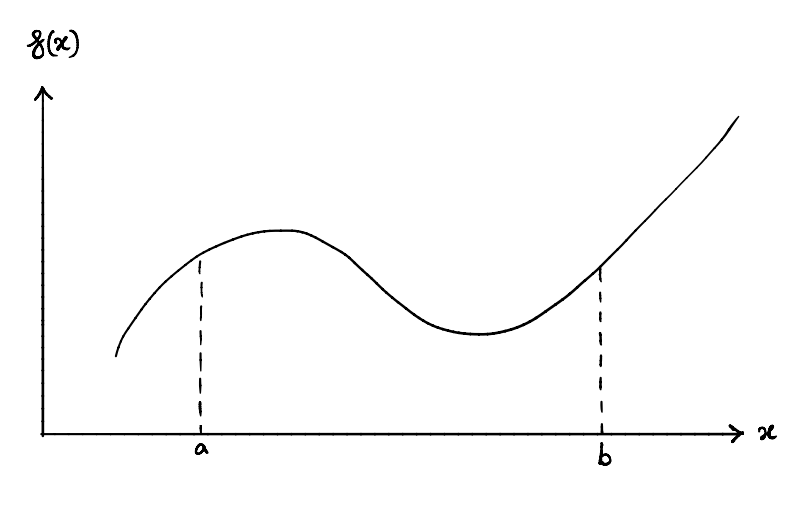
\includegraphics[scale=0.4]{images/fig1.png}
    \caption{Área debajo de la gráfica de $f$.}
    \label{fig:fig1}
\end{figure}

\begin{definition}[(El área bajo f)]
    Sea $f$ una función continua en $[a,b]$ no negativa y sea $\mathbb{A}:[a,b]\longrightarrow\mathbb{R}$ como sigue:
    $$\mathbb{A}(x) = \left\{
        \begin{array}{ll}
            0  & \mbox{si } x=a \\
            \\ \mbox{área acumulada bajo $f$ hasta $x$} & \mbox{si } x\in [a,b].
        \end{array}
    \right.$$
En esta definición, $\mathbb{A}(b)$ denota el área acumulada debajo de la gráfica de $f$ en el intervalo [a,b].
\end{definition}

$\mathbb{A}:[a,b]\longrightarrow\mathbb{R}$ satisface que:
\begin{enumerate}
    \item[a)] Por definición, $\mathbb{A}(a)=0$.
    \item[b)] Si $c\in [a,b]$, entonces $\mathbb{A}(a,b)=\mathbb{A}(a,c)+\mathbb{A}(c,b)$.
    \item[c)] Si $m$ es mínimo y $M$ es el máximo de la función en el intervalo $[a,b]$, entonces $m\leq f(x)\leq M$ y $m(b-a)\leq \mathbb{A}(b)\leq M(b-a)$, tal y como se muestra en la figura \ref{fig:fig2}.
\end{enumerate} 

\begin{figure}[h]
    \centering
    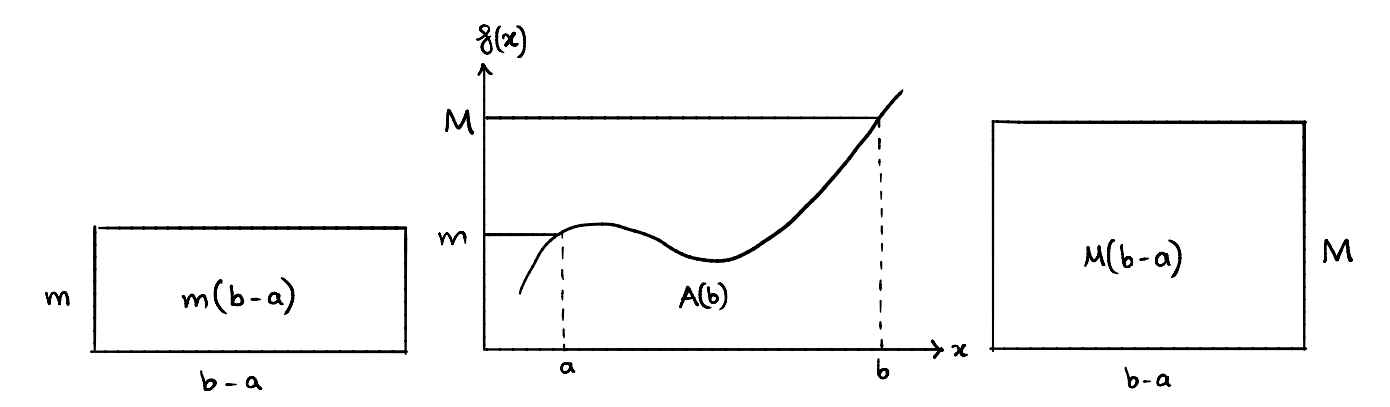
\includegraphics[scale=0.4]{images/fig2.png}
    \caption{Área debajo de la gráfica de $f$.}
    \label{fig:fig2}
\end{figure}

La notación integral: 

$$ \mathbb{A}(x)=\int_{a}^{x} \! {f(t)} \, \mathrm{dt} =
\left\{
    \begin{array}{ll}
        0  & \mbox{si } x=a \\
        \\ \mbox{área acumulada bajo $f$} & \mbox{si } x\in [a,b].
    \end{array}
\right.$$

\begin{example}[(Ejemplo ilustrativo)]
    Sea $I=[a,b]=[0,1]$ y $f(x)=x$, entonces $\exists c \in [0,1]$ tal que
    $$\integrate{a}{b}{f(x)}{x}=\integrate{0}{1}{f(x)}{x}=f(c)(b-a)=c(1-0)=c.$$
    \begin{figure}[h]
        \centering
        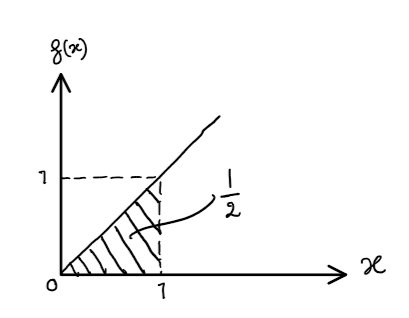
\includegraphics[scale=0.4]{images/fig2-1.png}
        \caption{Área debajo de la gráfica de $f$.}
        \label{fig:fig2-1}
    \end{figure}

    Es claro que el área acumulada es igual $\frac{1}{2}$. Entonces, en efecto, $\exists c \in [0,1]$ tal que
    $$f(c)(1-0)=f(c)=\integrate{0}{1}{f(x)}{x}=\frac{1}{2}\quad\Rightarrow\quad c=\frac{1}{2}.$$
\end{example}

\subsection{\col{El teorema del valor medio para integrales (TVMI)}}

\begin{theorem}[(Teorema del valor medio para integrales)]
    El teorema del valor medio para integrales ($TVMI$) estable que se si $f:[a,b]\longrightarrow\mathbb{R}$ es continua, entonces existe $c\in [a,b]$ tal que 
    $$\int_{a}^{b} \! {f(t)} \, \mathrm{dt}=f(c)(b-a).$$
\end{theorem}

\begin{proof}
    Sea $m$ y $M$ tal que $m\leq f(x)\leq M$ $\forall x\in [a,b]$, entonces
    $$ m(b-a)\leq \int_{a}^{b} \! {f(t)} \, \mathrm{dt}\leq M(b-a) $$ 
    $$ \Rightarrow m\leq \frac{\int_{a}^{b} \! {f(t)} \, \mathrm{dt}}{b-a}\leq M $$
    El teorema del valor medio de Bolzano establece que una función continua ``no se salta valores", entonces
    $$ f(s)=m\leq \frac{\int_{a}^{b} \! {f(t)} \, \mathrm{dt}}{b-a}\leq M=f(t) \quad \mbox{para algún} \quad s,t\in [a,b] $$
    $$ \Rightarrow f(c)=\frac{\int_{a}^{b} \! {f(t)} \, \mathrm{dt}}{b-a} \quad \mbox{para algún} \quad c\in [a,b] $$
    es decir, $f(c)=\frac{\int_{a}^{b} \! {f(t)} \, \mathrm{dt}}{b-a}$ es un valor que alcanza la función, pues $f(c)=\frac{\int_{a}^{b} \! {f(t)} \, \mathrm{dt}}{b-a}$ está entre el mínimo y el máximo.
    $$\Rightarrow f(c)(b-a)=\int_{a}^{b} \! {f(t)} \, \mathrm{dt} \quad \mbox{para algún} \quad c\in [a,b].$$
\end{proof}

\subsection{\col{El Teorema fundamental del cálculo (TFC)}}

\begin{theorem}[($TFC \#1$)]
    El teorema fundamental del cálculo parte 1 ($TFC \#1$) establece que si $f:[a,b]\longrightarrow\mathbb{R}$ es una función continua, entonces $\mathbb{A}(x)=\int_{a}^{x} \! {f(t)} \, \mathrm{dt}$ es una función continua y diferenciable tal que
    $$ \derivate{x}{\mathbb{A}(x)}=\derivate{x}{\int_{a}^{x} \! {f(t)} \, \mathrm{dt}}=f(x) $$
\end{theorem}

\begin{proof}
    \textbf{Caso 1.} ($h>0$)

    $$ \frac{d}{dx}\mathbb{A}(x)=\lim_{h\to 0}\frac{\mathbb{A}(x+h)-\mathbb{A}(x)}{h}= \lim_{h\to 0}\frac{  \int_{a}^{x+h} \! {f(t)} \, \mathrm{dt} - \int_{a}^{x} \! {f(t)} \, \mathrm{dt} }{h}$$
    $$= \lim_{h\to 0}\frac{  \int_{a}^{x} \! {f(t)} \, \mathrm{dt} + \int_{x}^{x+h} \! {f(t)} \, \mathrm{dt} - \int_{a}^{x} \! {f(t)} \, \mathrm{dt} }{h}=\lim_{h\to 0} \frac{\int_{x}^{x+h} \! {f(t)} \, \mathrm{dt}}{h} $$

    Por el teorema del valor medio para integrales, existe $c\in [x,x+h]$ tal que 

    $$\lim_{h\to 0} \frac{\int_{x}^{x+h} \! {f(t)} \, \mathrm{dt}}{h}=\lim_{h\to 0}\frac{f(c)(x+h-x)}{h}=\lim_{h\to 0}f(c)$$

    si $h>0$, entonces $x<x+h$ pero $c\in [x,x+h]$, de manera que si $h\longrightarrow 0^+$, entonces $c\longrightarrow x^+$, entonces $\lim_{h\to 0^+}f(c)=f(x)$, entonces $D^+(\mathbb{A}(x))=f(x)$

    \vspace{1cm}

    \textbf{Caso 2.} ($h<0$)

    $$ \frac{d}{dx}\mathbb{A}(x)=\lim_{h\to 0}\frac{\mathbb{A}(x+h)-\mathbb{A}(x)}{h}= \lim_{h\to 0}\frac{  \int_{a}^{x+h} \! {f(t)} \, \mathrm{dt} - \int_{a}^{x} \! {f(t)} \, \mathrm{dt} }{h}$$
    $$= \lim_{h\to 0}\frac{  \int_{a}^{x+h} \! {f(t)} \, \mathrm{dt} -\left( \int_{a}^{x+h} \! {f(t)} \, \mathrm{dt} + \int_{x+h}^{x} \! {f(t)} \, \mathrm{dt} \right)}{h}=\lim_{h\to 0} \frac{-\int_{x+h}^{x} \! {f(t)} \, \mathrm{dt}}{h} $$

    Por el teorema del valor medio para integrales, existe $c\in [x+h,x]$ tal que 

    $$\lim_{h\to 0} \frac{-\int_{x+h}^{x} \! {f(t)} \, \mathrm{dt}}{h}=\lim_{h\to 0}\frac{-f(c)(x-(x+h))}{h}=\lim_{h\to 0}f(c).$$

    Si $h<0$, entonces $x+h<x$ pero $c\in [x,x+h]$, de manera que si $h\longrightarrow 0^-$, entonces $c\longrightarrow x^-$, entonces $\lim_{h\to 0^-}f(c)=f(x)$, de manera que $D^-(\mathbb{A}(x))=f(x).$
    \vspace{0.3cm}
    Por el caso 1 y por el caso 2, se tiene que $D^+(\mathbb{A}(x))=f(x)$ y $D^-(\mathbb{A}(x))=f(x)$, entonces $\mathbb{A}'(x)=f(x)$.
    \vspace{0.3cm}
    \par Por el teorema fundamental del cálculo parte 1, vemos que el problema de hallar la función de área se convierte en hallar una primitiva de la función bajo la cual se quiere encontrar el área. 
\end{proof}

\begin{theorem}[($TFC \#2$)]
    El teorema fundamental del cálculo parte 2 ($TFC \#2$) establece que si $f:[a,b]\longrightarrow\mathbb{R}$ es una función continua, y $\derivate{x}{F(x)}=f(x)$, $\forall x\in [a,b]$, entonces 
    $$ \int_{a}^{b} \! {f(t)} \, \mathrm{dt}=F(b)-F(a)=F(t) \Big|_a^b $$ 
\end{theorem}

\begin{proof}
    Sea $G(x)=\int_{a}^{x} \! {f(t)} \, \mathrm{dt}$ y sea $F(x)$ tal que $F'(x)=f(x)$, antiderivadas de $f(x)$ (dos funciones cuyas derivadas son $f(x)$), entonces $F(x)$ y $G(x)$ difieren por una contante $C$:

    $$ F(x)=G(x)+C \quad \forall x\in [a,b].$$

    Ahora hacemos:

    $$\int_{a}^{b} \! {f(t)} \, \mathrm{dt}=\int_{a}^{b} \! {f(t)} \, \mathrm{dt}-0=\int_{a}^{b} \! {f(t)} \, \mathrm{dt}- \int_{a}^{a} \! {f(t)} \, \mathrm{dt}$$
    $$=G(b)-G(a)=G(b)+c-(G(a)+c)=F(b)-F(a).$$

    Por lo tanto, 

    $$.\int_{a}^{b} \! {f(t)} \, \mathrm{dt}=F(b)-F(a).$$
\end{proof}

\textbf{Convención:} si $b\leq a$, entonces $\int_{a}^{b} \! {f(t)} \, \mathrm{dt}=-\int_{b}^{a} \! {f(t)} \, \mathrm{dt}$.

\newpage

\vspace{1cm}

Se tiene que interpretar correctamente la definición de valor absoluto:  sean $a$ y $b$ tal que $a\leq b$. Si se tiene $\int_{a}^{b} \! {|t|} \, \mathrm{dt}$, entonces hay tres casos:

\vspace{0.5cm}

\textbf{Caso 1.} $b\leq 0$, entonces 
$$\int_{a}^{b} \! {|t|} \, \mathrm{dt}=\int_{a}^{b} \! {-t} \, \mathrm{dt}=-\int_{a}^{b} \! {t} \, \mathrm{dt}=-\frac{t^2}{2}\Big|_a^b=\frac{a^2-b^2}{2}>0.$$

\begin{figure}[h]
    \centering
    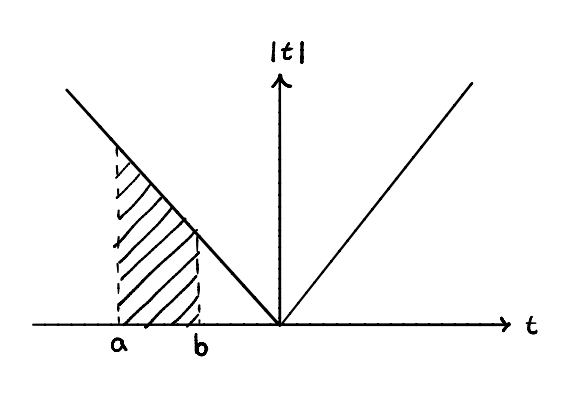
\includegraphics[scale=0.3]{images/fig3.png}
    \caption{Área debajo de la gráfica de $|t|$ caso 1.}
    \label{fig:fig3}
\end{figure}

\textbf{Caso 2.} $a\leq 0\leq b$, entonces
$$\int_{a}^{b} \! {|t|} \, \mathrm{dt}=\int_{a}^{0} \! {-t} \, \mathrm{dt}+\int_{0}^{b} \! {t} \, \mathrm{dt}=-\int_{a}^{0} \! {t} \, \mathrm{dt}+\int_{0}^{b} \! {t} \, \mathrm{dt}=-\frac{t^2}{2}\Big|_a^0+\frac{t^2}{2}\Big|_0^b=\frac{a^2+b^2}{2}>0.$$

\begin{figure}[h]
    \centering
    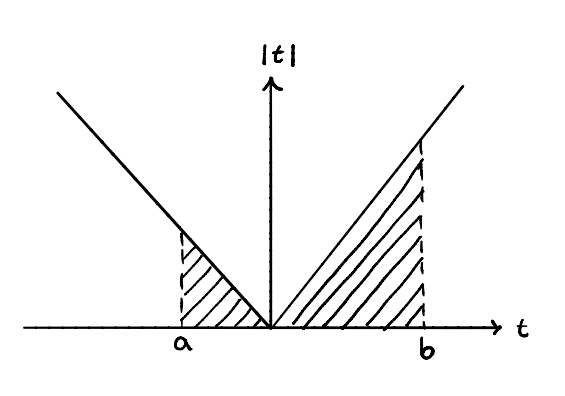
\includegraphics[scale=0.3]{images/fig4.png}
    \caption{Área debajo de la gráfica de $|t|$ caso 2.}
    \label{fig:fig4}
\end{figure}

\textbf{Caso 3.} $a\geq 0$, entonces 
$$\int_{a}^{b} \! {|t|} \, \mathrm{dt}=\int_{a}^{b} \! {t} \, \mathrm{dt}=\frac{t^2}{2}\Big|_a^b=\frac{b^2-a^2}{2}>0.$$

\begin{figure}[h]
    \centering
    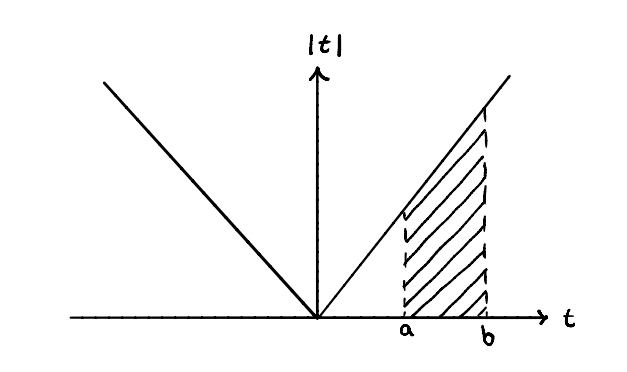
\includegraphics[scale=0.3]{images/fig5.png}
    \caption{Área debajo de la gráfica de $|t|$ caso 3.}
    \label{fig:fig5}
\end{figure}

Los tres casos anteriores surge de interpretar correctamente la definicion de valor absoluto:

$$|x|=\left\{
    \begin{array}{ll}
        x  & \mbox{si } x\geq 0\\
        -x & \mbox{si } x<0.
    \end{array}
\right.$$

\newpage

\section{\col{El logaritmo natural}}

\subsection{\col{Propiedades del logaritmo natural}}

La regla del exponente dice que $\int_{}^{} \! {t^r} \, \mathrm{dt}=\frac{t^{r+1}}{r+1}+C$, $\forall r\neq -1$. ¿Qué pasa si $r=-1$? La respuesta es que en este caso no se puede aplicar la regla del exponente, entonces se tiene que hallar una función diferenciable $L(x)$ tal que 

$$ L'(x)=x^{-1}=\frac{1}{x} \quad \forall x\neq 0 $$

\begin{definition}
    El logaritmo natural es una función $ln:\mathbb{R^+}\longrightarrow\mathbb{R}$ definida como sigue:
    $$ \ln(x)=\xinteg{1}{x}{\frac{1}{t}}{dt}=\xinteg{1}{x}{t^{-1}}{dt}.$$
    El logaritmo natural es el área debajo de la gráfica de la función $f(x)=\frac{1}{x}$ en el intervalo $[1,a]$:
    
    \begin{figure}[h]
        \centering
        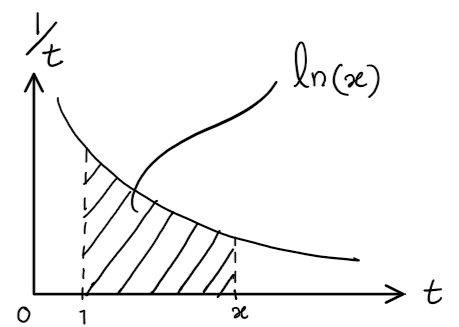
\includegraphics[scale=0.4]{images/fig6.png}
        \caption{$ln(x)$ = Área debajo de la gráfica de $\frac{1}{t}$ desde 1 hasta $x$.}
        \label{fig:fig6}
    \end{figure}
\end{definition}

\textbf{Observacion:} Por el TFC \#1, $\derivate{x}{\ln(x)}=   \derivate{x}{\xinteg{1}{x}{\frac{1}{t}}{dt}}=\frac{1}{x}$.

Sea $F(t)=\ln(-t)+C$ y $G(t)=\ln(t)+C$, entonces $\frac{d}{dt}F(t)=\frac{1}{t}$ y $\frac{d}{dt}G(f)=\frac{1}{t}$, entonces se sigue que 

$$ \xinteg{}{}{\frac{1}{t}}{dt}= \left\{
    \begin{array}{ll}
        \ln(-t)+C  & \mbox{si } t<0 \\
        \\ \ln(t)+C & \mbox{si } t>0
    \end{array}
\right.$$

Por lo tanto $\xinteg{}{}{\frac{1}{t}}{dt}=\ln|t|+C$ si $t\neq 0$. En general, $\xinteg{}{}{\frac{u'}{u}}{du}=\ln|u|+C$ si $u\neq 0$.

\begin{theorem}[(Propiedades del logaritmo natural)]
    $\forall a,b>0$ y $\forall r\in\mathbb{Q}$ ocurre que:
    \begin{enumerate}
        \item[a)] $\ln(ab)=\ln(a)+\ln(b)$
        \item[b)] $\ln(a^{-1})=\ln\left(\frac{1}{a}\right)=-\ln(a)$
        \item[c)] $\ln\left(\frac{a}{b}\right)=\ln(a)-\ln(b)$
        \item[d)] $\ln(a^r)=r\ln(a)$
    \end{enumerate}
\end{theorem}

\begin{proof}
    \begin{enumerate}
    \item[a)] \textbf{Por demostrar:} $\ln(ab)=\ln(a)+\ln(b)$
    
    Sea $f(b)=\ln(ab)\Rightarrow\frac{d}{db}f(b)=\frac{1}{b}$. Sea $g(b)=\ln(b)\Rightarrow\frac{d}{db}g(b)=\frac{1}{b}$, entonces $f(b)$ y $g(b)$ tienen la misma derivada, por lo tanto, difieren por una contante $C$, $\forall b\in (0,\infty)$, si y sólo si $F(b)=G(b)+C$, $\forall b\in (0,\infty)$. Si $b=1\Rightarrow F(1)=G(1)+C=\ln(1)+C=0+C=C \Leftrightarrow F(1)=C$, pero $F(1)=\ln(a(1))=\ln(a)\Leftrightarrow F(1)=C=\ln(a)\Leftrightarrow C=\ln(a)\Leftrightarrow F(b)=\ln(b)+\ln(a)=\ln(a)+\ln(b) \therefore \ln(ab)=\ln(a)+\ln(b) \quad \forall b\in (0,\infty)$.
    
    \item[b)] \textbf{Por demostrar:} $\ln(a^{-1})=\ln\left(\frac{1}{a}\right)=-\ln(a)$
    
    Si $b>0\Leftrightarrow\frac{1}{b}>0$. $1=\frac{b}{b}\Leftrightarrow 1=bb^{-1}\Leftrightarrow\ln(1)=\ln(bb^{-1})\Leftrightarrow 0=\ln(bb^{-1})\Leftrightarrow 0=\ln(b)+ln(b^{-1})\Leftrightarrow \ln(b^-1)=-\ln(b)$. 
    
    \item[c)] \textbf{Por demostrar:} $\ln\left(\frac{a}{b}\right)=\ln(a)-\ln(b)$
    
    $\ln\left(\frac{a}{b}\right)=\ln(ab^{-1})=\ln(a)+\ln(b^{-1})=\ln(a)-\ln(b)$.
    
    \item[d)] \textbf{Por demostrar:} $\ln(a^r)=r\ln(a)$
    
    Sea $F(a)=\ln(a^{r})\Rightarrow \frac{d}{da}F(a)=\frac{r}{a}$. Sea $G(a)=r\ln(a)\Rightarrow\frac{d}{da}G(a)=\frac{r}{a}$, entonces $F(a)$ y $G(a)$ tienen la misma derivada, por lo tanto, difieren por una constante $C$, $\forall a\in (0,\infty)$, si y sólo si $F(a)=G(a)+C$, $\forall a\in (0,\infty)$.
    
    Si $a=1 \Rightarrow F(1)=G(1)+C=r\ln(1)+C=0+C=C\Leftrightarrow F(1)=C$, pero $F(1)=\ln(1^{r})=\ln(1)=0\Leftrightarrow C=0\Leftrightarrow F(a)=G(a)\Leftrightarrow r\ln(a)=\ln(a^r)\Leftrightarrow \ln(a^r)=r\ln(a)$. 
    
    \end{enumerate}    
\end{proof}


En las demostraciones anteriores se usó el hecho de que dos funciones que tiene la misma derivada difieren por una constante.


\subsection{\col{Límites relevantes del logaritmo natural}}

Los siguientes teoremas serán de gran utilidad para conocer el comportamiento del logaritmo natural y su gráfica.

\begin{theorem}
    $\lim_{x\to \infty}\ln(x)=\infty$.
\end{theorem}

\begin{proof}
    Se prueba por inducción que $\sum_{i=1}^{2^n}\frac{1}{i}\geq 1+\frac{n}{2}$. Además, $\lim_{n\to \infty}\left(a+\frac{n}{2}\right)=\infty$, entonces
    $$\lim_{n\to \infty}\sum_{i=1}^{2^n}\frac{1}{i}=\infty.$$
    Luego, se observa que, $\forall n>1$, $(1)\frac{1}{2}+(1)\frac{1}{3}+\cdots+(1)\frac{1}{n}<\ln(n)$, tal y como se muestra en la siguiente gráfica:
    \begin{figure}[H]
        \centering
        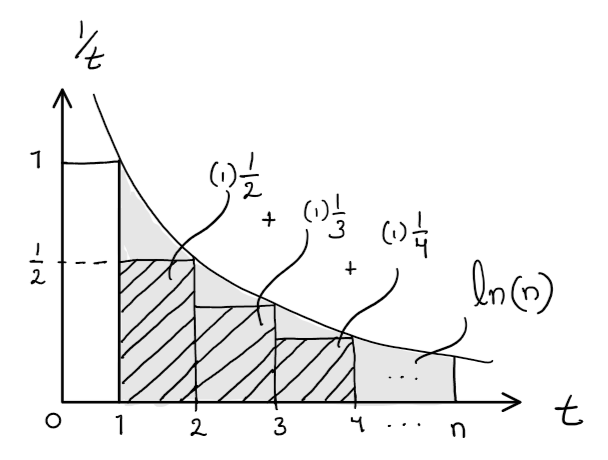
\includegraphics[scale=0.4]{images/fig7.png}
        \caption{Claramente el área sombreada es mayor al área rayada.}
        \label{fig:fig5}
    \end{figure}
    Entonces $\forall n>1$, $(1)\frac{1}{2}+(1)\frac{1}{3}+\cdots+(1)\frac{1}{n}<\ln(n)$, así pues 
    $$\frac{1}{2}+\frac{1}{3}+\cdots+\frac{1}{n}<\ln(n)$$
    $$\Leftrightarrow \quad \left(1+\frac{1}{2}+\frac{1}{3}+\cdots+\frac{1}{n}\right)-1<\ln(n)$$
    $$\Leftrightarrow \quad \lim_{n\to \infty}\left(1+\frac{1}{2}+\frac{1}{3}+\cdots+\frac{1}{n}\right)-1 <\lim_{n\to\infty}\ln(n).$$
    Se sigue que $\lim_{n\to \infty}\left(\sum_{i=1}^{2^n}\frac{1}{i}-1\right)<\lim_{n\to\infty}\ln(n)$, entonces $\infty=\lim_{n\to \infty}\left(\sum_{i=1}^{2^n}\frac{1}{i}-1\right)<\lim_{n\to\infty}\ln(n)$, por lo tanto $\lim_{x\to\infty}\ln(x)=\infty$.
\end{proof}

\begin{theorem}
    $\lim_{x\to 0^+}\ln(x)=-\infty$.
\end{theorem}

\begin{proof}
    Sea $t=\frac{1}{x}$. Si $x\to 0^+$, entonces $t\to\infty$, además, si $t\to\infty$, entonces $x\to 0^+$, por lo tanto, $t\to\infty$, si y sólo si $x\to 0^+$. De manera que
    $$\lim_{x\to 0^+}\ln(x)=\lim_{t\to\infty}\ln\left(\frac{1}{t}\right)=\lim_{t\to\infty}\ln(t^{-1})=\lim_{t\to\infty}-\ln(t)=-\lim_{t\to\infty}\ln(t)=-\infty.$$
\end{proof}

\begin{theorem}
    $\lim_{x\to\infty}\frac{\ln(x)}{x}=0$.
\end{theorem}

\begin{proof}
    Si $1\leq t$, entonces $t\leq t^2$, entonces $\sqrt{t}\leq \sqrt{t^2}$, entonces $\sqrt{t}\leq t$, entonces $\frac{1}{\sqrt{t}}\geq\frac{1}{t}$, tal y como se muestra en la siguiente gráfica:
    \begin{figure}[H]
        \centering
        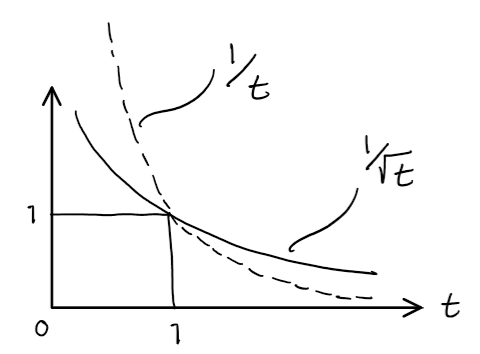
\includegraphics[scale=0.4]{images/fig8.png}
        \caption{Claramente el área sombreada es mayor al área rayada.}
        \label{fig:fig5}
    \end{figure}    
    Por lo tanto, si $x\geq 1$, entonces $ln(x)=\xinteg{1}{x}{\frac{1}{t}}{dt}\leq\xinteg{1}{x}{\frac{1}{\sqrt{t}}}{dt}=2\sqrt{x}-2<2\sqrt{x}$, entonces $\ln(x)<2\sqrt{x}$. Por lo tanto, $0<\ln(x)<2\sqrt{x} \quad \forall x\geq 1$, entonces $0<\frac{\ln(x)}{x}<\frac{2\sqrt{x}}{x}$, entonces $\lim_{x\to\infty}0<\lim_{x\to\infty}\frac{\ln(x)}{x}<\lim_{x\to\infty}\frac{2\sqrt{x}}{x}$, entonces $0<\lim_{x\to\infty}\frac{\ln(x)}{x}<0$, entonces $\lim_{x\to\infty}\frac{\ln(x)}{x}=0.$
\end{proof}

\begin{theorem}
    Si $a$ y $b$ con constantes, entonces $\lim_{x\to\infty}\frac{\ln(x)}{ax+b}=0.$
\end{theorem}

\begin{proof}
    $$ \lim_{x\to\infty}\frac{\ln(x)}{ax+b}=\lim_{x\to\infty}\frac{\frac{\ln(x)}{x}}{\frac{ax+b}{x}}=\frac{\lim_{x\to\infty}\frac{\ln(x)}{x}}{\lim_{x\to\infty}\frac{ax+b}{x}}=\frac{0}{a+0}=0.$$
\end{proof}

\subsection{\col{La gráfica de la función logaritmo natural}}

A continuación se trazará con todo detalle la gráfica de la función logaritmo natural enunciando todas sus propiedades: 0) Dominio, imagen y puntos por los que pasa la función; 1) Primera derivada, intervalos de crecimiento y decrecimiento, y puntos críticos estacionarios o puntos singulares; 2) Segunda derivada, intervalos de concavidad positiva y negativa, y puntos de inflexión; 3) Límites relevantes y comportamiento asintótico. 

\begin{enumerate}
    \item[0)] $Dom(\ln)=(0,\infty)$, $Img(\ln)=(-\infty,\infty)$ y Pasa por los puntos $(1,0)$ y $(e,1)$.
    \item[1)] $\ln'(x)=\frac{1}{x}>0 \quad \forall x\in (0,\infty)$. Por lo tanto:
    \begin{enumerate}
    \item Intervalo de crecimiento$=(0,\infty)$
    \item Intervalo de decrecimiento$=\varnothing$
    \item No existen puntos críticos estacionarios
    \end{enumerate} 
    \item[2)] $\ln''(x)=-\frac{1}{x^2}<0 \quad \forall x\in (0,\infty)$. Por lo tanto:
    \begin{enumerate}
    \item Intervalo de concavidad positiva$=\varnothing$
    \item Intervalo de concavidad negativa$=(0,\infty)$
    \item No existen puntos de inflexión
    \end{enumerate}
    \item[3)] $\lim_{x\to\infty}\ln(x)=\infty$, $\lim_{x\to 0^+}\ln(x)=-\infty$, $\lim_{x\to\infty}\frac{\ln(x)}{x}=0$. Por lo tanto hay una asíntota vertical en $x=0$.
\end{enumerate}

Dado lo anterior, la gráfica de la función logaritmo natural tiene el siguiente aspecto:

\begin{figure}[H]
    \centering
    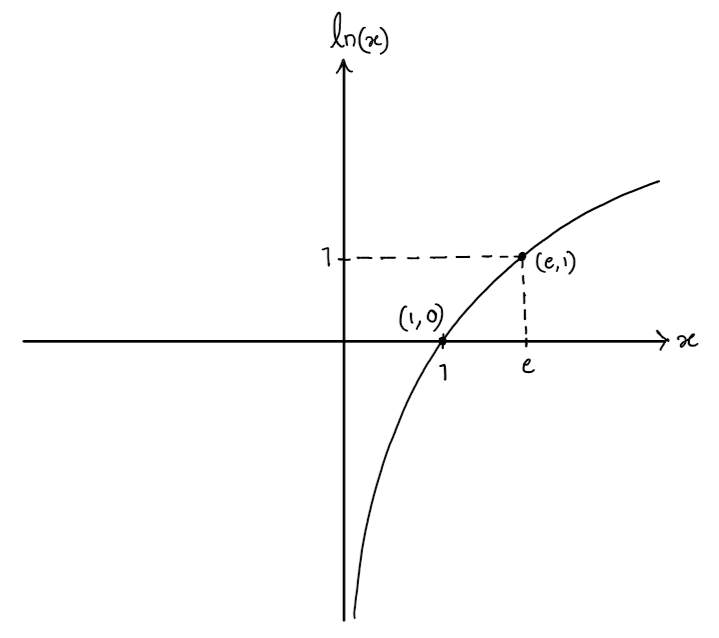
\includegraphics[scale=0.4]{images/fig9.png}
    \caption{Gráfica de la función logaritmo natural.}
    \label{fig:fig9}
\end{figure}    

\subsection{\col{Algunos límites importantes}}

\begin{theorem}
    $\lim_{x\to 0^+}\frac{\ln(x)}{x}=-\infty$.
\end{theorem}

\begin{proof}
    $$\lim_{x\to 0^+}\frac{\ln(x)}{x}=\lim_{x\to 0^+}\ln(x)\left(\frac{1}{x}\right)="\infty\cdot-\infty"=-\infty.$$
\end{proof}

\begin{theorem}
    $\lim_{x\to 0^+}x\ln(x)=0$.
\end{theorem}

\begin{proof}
    Sea $t=\frac{1}{x}$. Si $x\to 0^+$, entonces $t\to\infty$, además, si $t\to\infty$, entonces $x\to 0^+$, por lo tanto, $t\to\infty$, si y sólo si $x\to 0^+$. De manera que
    $$\lim_{x\to 0^+}x\ln(x)=\lim_{t\to\infty}\frac{\ln\left(\frac{1}{t}\right)}{t}=\lim_{t\to\infty}-\frac{\ln(t)}{t}=-0=0.$$
\end{proof}

\begin{theorem}
    $\lim_{x\to\infty}\frac{\ln(1+x^2)}{x}=0$.
\end{theorem}

\begin{proof}
    Si $a<b<c$, entonces $\ln(a)<\ln(b)<\ln(c)$, por lo que $\ln(x^2)<\ln(1+x^2)<\ln(x^2+x^2)$, de manera que $2\ln(x)<\ln(1+x^2)<\ln(2x^2)$, así pues $2\ln(x)<\ln(1+x^2)<\ln(2)+\ln(x^2)$, entonces $\frac{2\ln(x)}{x}<\frac{\ln(1+x^2)}{x}<\frac{\ln(2)+\ln(x^2)}{x}$, se sigue que $\lim_{x\to\infty}\frac{2\ln(x)}{x}<\lim_{x\to\infty}\frac{\ln(1+x^2)}{x}<\lim_{x\to\infty}\frac{\ln(2)+\ln(x^2)}{x}$, de ahí que $0<\lim_{x\to\infty}\frac{\ln(1+x^2)}{x}<0$, por lo tanto $\lim_{x\to\infty}\frac{\ln(1+x^2)}{x}=0$.
\end{proof}

\subsection{\col{Primitivas trigonométricas}}

Con el material cubierto hasta este punto, se pueden hallar las primivitvas de las principales funciones trigonométricas. 

\vspace{0.5cm}

Recordar que $\xinteg{}{}{\frac{u'}{u}}{du}=\ln|u|+C$.

\vspace{0.5cm}

Las primitivas de las principales funciones trigonométricas son las siguientes:

\begin{enumerate}
    \item $$\xinteg{}{}{\sin(t)}{dt}=-\cos(t)+C$$
    \item $$\xinteg{}{}{\cos(t)}{dt}=\sin(t)+C$$
    \item $$\xinteg{}{}{\tan(t)}{dt}=\xinteg{}{}{\frac{\sin(t)}{\cos(t)}}{dt}=-\xinteg{}{}{\frac{-\sin(t)}{\cos(t)}}{dt}=-\xinteg{}{}{\frac{\cos'(t)}{\cos(t)}}{dt}=-\ln|\cos(t)|+C$$
    \item $$\xinteg{}{}{\cot(t)}{dt}=\xinteg{}{}{\frac{\cos(t)}{\sin(t)}}{dt}=\xinteg{}{}{\frac{\sin'(t)}{\cos(t)}}{dt}=\ln|\sin(t)|+C$$
    \item 
    $$\begin{aligned}
        \xinteg{}{}{\sec(t)}{dt} & = \xinteg{}{}{\sec(t)\frac{\sec(t)+\tan(t)}{\sec(t)+\tan(t)}}{dt}=\xinteg{}{}{\frac{\sec^2(t)+\sec(t)\tan(t)}{\sec(t)+\tan(t)}}{dt}  \\
        & = \xinteg{}{}{\frac{(\sec(t)+\tan(t))'}{\sec(t)+\tan(t)}}{dt}=\ln|\sec(t)+\tan(t)|+C \\
    \end{aligned}$$

    \item 
    $$\begin{aligned}
        \xinteg{}{}{\csc(t)}{dt} & = \xinteg{}{}{\csc(t)\frac{\cot(t)-\csc(t)}{\cot(t)-\csc(t)}}{dt}=\xinteg{}{}{\frac{\csc(t)\cot(t)-\csc^2(t)}{\cot(t)-\csc(t)}}{dt} \\
        & = \xinteg{}{}{\frac{(\cot(t)-\csc(t))'}{\cot(t)-\csc(t)}}{dt}=\ln|\cot(t)-\csc(t)|+C. \\
    \end{aligned}$$
\end{enumerate}

\vspace{0.5cm}

\subsection{\col{Diferenciación logarítmica}}

Cuando se tiene una función muy ``exótica", en algunas ocaciones, es más conveniente utilizar la diferenciación logarítmica.

\begin{theorem}
    Sea $y=f(x)$, entonces $y'=y(\ln(f(x)))'$.
\end{theorem}

\begin{proof}
    Si $y=f(x)$, entonces $\ln(y)=\ln(f(x))$, de manera que $\frac{d}{dx}\ln(y)=\frac{d}{dx}\ln(f(x))$, así pues, $\frac{y'}{y}=(\ln(f(x)))'$, por lo tanto $y'=y(\ln(f(x)))'$.
\end{proof}

\subsection{\col{Ejercicios}}

\begin{enumerate}
    \item Demuestre que $5\leq \integrate{-3}{2}{\sqrt{t^2+1}}{t}\leq 5\sqrt{10}$.
    \item Sea $f:[-2,13]\to\mathbb{R}$ continue y suponga que $30 \leq \integrate{-2}{13}{f(t)}{t}$. Demuestre que existe una $c\in[-2,13]$ tal que $f(c)\geq 2$.
    \item Sea $T(x)=\integrate{0}{x}{f(t)}{t}$, $f(t)=\frac{1}{1+t^2}$. Demuestre que
        \begin{enumerate}
            \item $T'(x)\geq 0$ y $T$ es concava hacia abajo en $(-\infty,0]$
            \item $T$ es concava hacia arriba en $[0,\infty]$
            \item $T$ tiene un punto de inflexión en $x=0$
        \end{enumerate}
    \item Encuentre el área sombreada
        \begin{figure}[H]
            \centering
            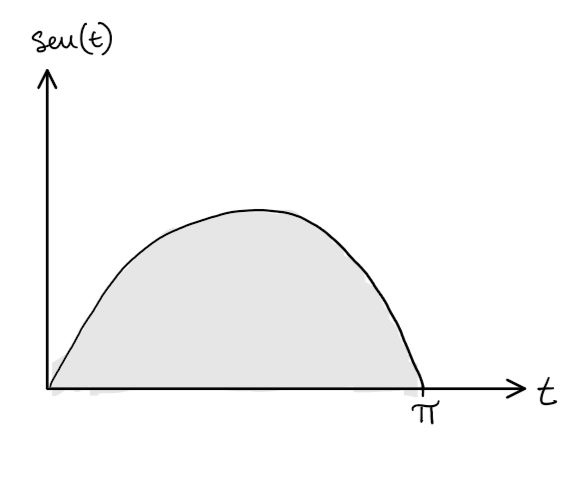
\includegraphics[scale=0.4]{images/fig10.png}
            \caption{Hallar el área sombreada.}
            \label{fig:fig10}
        \end{figure}  
    \item Resulva las siguientes integrales:
        %\setlength{\columnsep}{-0.6in}
        \begin{multicols}{2}
            \begin{enumerate}
                \item $\integrate{9}{64}{\frac{1}{\sqrt{t}\sqrt{1+\sqrt{t}}}}{t}$
                \item $\integrate{-5}{12}{\sqrt{4+|t|}}{t}$
            \end{enumerate}
        \end{multicols}
    \item Obtén $\integrate{a}{b}{|x|}{x}$ si
        %\setlength{\columnsep}{-0.6in}
        \begin{multicols}{3}
            \begin{enumerate}
                \item $b<0$
                \item $b>0$ y $a<0$
                \item $a>0$
            \end{enumerate}
        \end{multicols}
    \item Simplifique y resuelva $\ln{\left(\frac{A^{\frac{3}{2}}B^6}{\sqrt{A}B^{\frac{5}{7}}}\right)^{-\frac{1}{3}}}$.
    \item Calcule $\eval{\frac{d}{dx}\left(\frac{\sqrt{x^2+1}(x^2+4)^{37}}{(4x^2+7)^{\frac{1}{3}}}\right)^{\frac{1}{3}}}_{x=0}$.
    \item Calcule y grafique el área calculada en las siguientes integrales:
        \begin{multicols}{4}
            \begin{enumerate}
                \item $\integrate{-2}{-\frac{3}{2}}{\frac{1}{1+t}}{t}$
                \item $\integrate{\frac{\pi}{4}}{\frac{\pi}{3}}{\cot(t)}{t}$
                \item $\integrate{2}{5}{\frac{1}{t\ln (t)}}{t}$
                \item $\integrate{\pi}{\frac{5\pi}{4}}{\sec (t)}{t}$
            \end{enumerate}
        \end{multicols}
    \item Calcula lo siguiente:
        \begin{multicols}{2}
            \begin{enumerate}
                \item $x\ln(e)$
                \item $\ln(e^x)$
            \end{enumerate}
        \end{multicols}
    \item Trace con todo detalle la gáfica de las siguientes funciones:
        \begin{multicols}{3}
            \begin{enumerate}
                \item $f(x)=\frac{\ln(x)}{x}$
                \item $f(x)=x\ln(x)$
                \item $f(x)=\ln(1+x^2)$
            \end{enumerate}
        \end{multicols}
\end{enumerate}

\newpage

\section{\col{La exponencial}}

\subsection{\col{Propiedades de la exponencial}}

Trazando la gráfica de la función del logaritmo natural, se probó que $\ln:(0,\infty)\longrightarrow\mathbb{R}$ es una función inyectiva y suprayectiva, y por lo tanto, $\ln(x)$ es una función biyectiva. Se puede concluir entonces que $\ln(x)$ tiene función inversa, es decir, $\ln(x)$ es invertible.

\begin{definition}[(La función exponencial)]
    La exponencial es una función $\exp:\mathbb{R}\longrightarrow (0,\infty)$ y se define como la inversa bajo composición de la función del logaritmo natural. De manera que 
    $$ y=\ln(x), \quad \mbox{si y sólo si} \quad x=\exp(y).$$
\end{definition}

Se puede obtener la función exponencial a partir de la inversa de la función $\ln(x)$. Para esto, se tiene que hacer una reflexión de $\ln(x)$ con respecto al origen tal y como se muestra en la siguiente figura:

\begin{figure}[H]
    \centering
    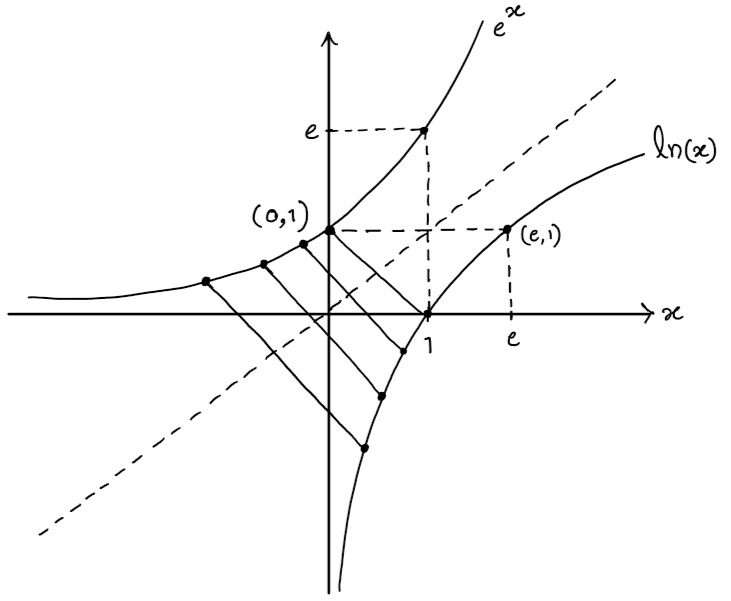
\includegraphics[scale=0.4]{images/fig11.png}
    \caption{Reflexión con respecto a la identidad de la función $\ln(x)$.}
    \label{fig:fig11}
\end{figure}

\begin{theorem}
    Si $f(x)$ es una función estrictamente creciente tal que existe su inversa, entonces $f^{-1}(x)$ es una función estrictamente creciente, es decir, la inversa de una función creciente es una función creciente.
\end{theorem}

\begin{proof}
    Sea $a<b$. Supongamos que $f^{-1}(a)\geq f^{-1}(b)$, entonces, como $f(x)$ es una función creciente, $f(f^{-1}(a))\geq f(f^{-1}(b))$, entonces $a\geq b$, lo cual es una contradicción, por lo tanto, por reducción a lo absurdo, tiene que suceder que $f^{-1}(a)<f^{-1}(b)$.
\end{proof}

\begin{theorem}[(Propiedades de la exponencial)]
    $\forall a,b\in\mathbb{R}$ y $\forall r\in\mathbb{Q}$ ocurre que:
    \begin{multicols}{2}
        \begin{enumerate}
            \item[a)] $\exp(a+b)=\exp(a)\exp(b)$
            \item[b)] $\exp(a-b)=\frac{\exp(a)}{\exp(b)}$
            \item[c)] $\exp(-b)=\frac{1}{\exp(b)}=(\exp(b))^{-1}$
            \item[d)] $\exp(ra)=(\exp(a))^r$
        \end{enumerate}
    \end{multicols}
\end{theorem}

\begin{proof}
    \begin{enumerate}
        \item[a)] \textbf{Por demostrar:} $\exp(a+b)=\exp(a)\exp(b)$
        
        Sea $x=\exp(a)$ y $y=\exp(b)$, entonces $a=\ln(x)$ y $b=\ln(y)$, luego $\ln(xy)=\ln(x)+\ln(y)=a+b$, 
        así pues, $\ln(xy)=a+b$, de manera que $\exp(\ln(xy))=\exp(a+b)$, se sigue que $xy=\exp(a+b)$, por lo tanto $\exp(a+b)=\exp(a)\exp(b)$.
        
        \item[b)] \textbf{Por demostrar:} $\exp(a-b)=\frac{\exp(a)}{\exp(b)}$
        
        Sea $x=\exp(a)$ y $y=\exp(b)$, entonces $a=\ln(x)$ y $b=\ln(y)$, luego $\ln\left(\frac{x}{y}\right)=\ln(x)-\ln(y)=a-b$, así pues $\ln\left(\frac{x}{y}\right)=a-b$, de manera que $\exp\left(\ln\left(\frac{x}{y}\right)\right)=\exp(a-b)$, se sique que $\frac{x}{y}=\exp(a-b)$, por lo tanto $\exp(a-b)=\frac{\exp(a)}{\exp(b)}$.
        
        \item[c)] \textbf{Por demostrar:} $\exp(-a)=\frac{1}{\exp(a)}=(\exp(a))^{-1}$
        
        Sea $x=\exp(a)$, entonces $a=\ln(x)$, luego $\ln\left(\frac{1}{x}\right)=\ln(x^{-1})=-\ln(x)=-a$, así pues $\ln\left(\frac{1}{x}\right)=-a$, de manera que $\exp\left(\ln\left(\frac{1}{x}\right)\right)=\exp(-a)$, se sique que $\frac{1}{x}=\exp(-a)$, por lo tanto $\exp(-a)=\frac{1}{\exp(a)}=(\exp(a))^{-1}$.
        
        \item[d)] \textbf{Por demostrar:} $\exp(ra)=(\exp(a))^r$
        
        Sea $x=\exp(a)$, entonces $a=\ln(x)$, luego $\ln(x^r)=r\ln(x)$, así pues $\exp(\ln(x^r))=\exp(r\ln(x))$, de manera que $x^r=\exp(r\ln(x))$, se sigue que $\exp(ra)=(\exp(a))^{r}$.
        
    \end{enumerate}
\end{proof}

\subsection{\col{Límites relevantes de la exponencial}}

\begin{theorem}
    $\ln(x)\leq x-1 \quad \forall x\geq 1$.
\end{theorem}

\begin{proof}
    Gráficamente, se puede observar que el área del rectángulo dada por $x-1$ es mayor al área sombreada dada por $\ln(x)=\integrate{1}{x}{\frac{1}{t}}{t}$:
    \begin{figure}[H]
        \centering
        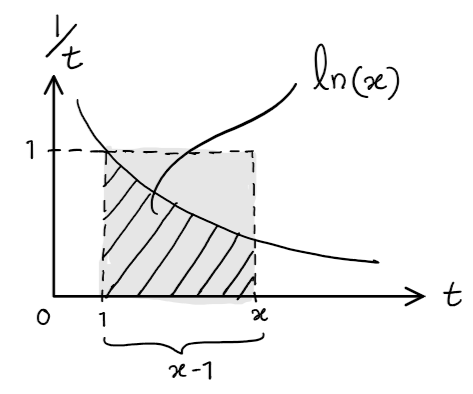
\includegraphics[scale=0.4]{images/fig12.png}
        \caption{Note que el área sombreada es mayor al área rayada.}
        \label{fig:fig12}
    \end{figure}
    Por el teorema del valor medio para integrales, se tiene que existe algúna $c\in [1,x]$ tal que
    $$\ln(x)=\xinteg{1}{x}{\frac{1}{t}}{dt}=f(c)(x-1)=\frac{1}{c}(x-1).$$
    Si $c=1$, entonces $\ln(x)=x-1$, pero si $c=x$, entonces $\ln(x)=\frac{x-1}{x}$. Además, si $x\geq 1$ se tiene que 
    $$ (x-1)^2=x^2-2x-1\geq 0 \quad \Rightarrow \quad x^2-2x\geq 1 \quad \Rightarrow \quad x^2-x\geq 1+x $$
    $$ \Rightarrow\quad x(x-1)\geq 1+x \quad\Rightarrow \quad x-1\geq \frac{1+x}{x} \geq \frac{x-1}{x} $$
    Se sigue del teorema del valor medio para integrales que $\frac{x-1}{x}\leq\ln(x)\leq x-1$. En particular se tiene que $\ln(x)\leq x-1$.
\end{proof}

\begin{theorem}
    $\lim_{x\to \infty}\exp(x)=\infty$.
\end{theorem}

\begin{proof}
    Si $x\geq 1$, entonces $\ln(x)\leq x-1\leq x$, como la función esponencial es una función creciente, se tiene que $\exp(\ln(x))\leq\exp(x)$, se sigue que $x\leq\exp(x)$, de manera que
    $$ \lim_{x\to\infty}x\leq\lim_{x\to\infty}\exp(x)\quad\Rightarrow\quad \infty\leq\lim_{x\to\infty}\exp(x) $$
    $$ \therefore \quad\lim_{x\to\infty}\exp(x)=\infty.$$
\end{proof}

\begin{theorem}
    $\lim_{x\to -\infty}\exp(x)=0$.
\end{theorem}

\begin{proof}
    Sea $t=-x$. Si $x\to -\infty$, entonces $t\to\infty$, además, si $t\to\infty$, entonces $x\to-\infty$, por lo tanto, $x\to -\infty$, si y sólo si $t\to\infty$. De manera que
    $$\lim_{x\to -\infty}\exp(x)=\lim_{t\to\infty}\exp(-t)=\lim_{t\to\infty}\frac{1}{\exp(t)}=``0^+"=0.$$
\end{proof}

\begin{theorem}
    $\lim_{x\to\infty}\frac{x}{\exp(x)}=0$.
\end{theorem}

\begin{proof}
    Sea $t=\exp(x)$. Si $x\to\infty$, entonces $t\to\infty$, además, si $t\to\infty$, entonces $x\to\infty$, por lo tanto, $x\to\infty$, si y sólo si $t\to\infty$. De manera que
    $$ \lim_{x\to\infty}\frac{x}{\exp(x)}=\lim_{t\to\infty}\frac{\ln(t)}{t}=0.$$
\end{proof}

\begin{theorem}
    Si $a$ y $b$ son constantes, entonces $\lim_{x\to\infty}\frac{ax+b}{\exp(x)}=0.$
\end{theorem}

\begin{proof}
    $$\begin{aligned}
        \lim_{x\to\infty}\frac{ax+b}{\exp(x)} & = \lim_{x\to\infty}\left( \frac{ax}{\exp(x)}+\frac{b}{\exp(x)} \right)=\lim_{x\to\infty}\frac{ax}{\exp(x)}+\lim_{x\to\infty}\frac{b}{\exp(x)} \\
        & = a\lim_{x\to\infty}\frac{x}{\exp(x)}+b\lim_{x\to\infty}\frac{1}{\exp(x)}=a(0)+b(0)=0. \\
    \end{aligned}$$
\end{proof} 

Por el teorema anterior, se puede conlcuir que la función exponencial no tiene asíntotas oblícuas.

\subsection{\col{La gráfica de la función exponencial}}

Para trazar la gráfica de la funcion exponencial, primero será necesario probar que la función $\exp(x)$ es diferenciable.

\begin{theorem}
    La función exponencial $\exp(x)$ es diferenciable en $\mathbb{R}$ y $\exp'(x)=\exp(x)$.
\end{theorem}

\begin{proof}    
    Dado que la función exponencial es la inversa de la función logaritmo, se tiene lo siguiente:

    $$ \ln(\exp(x))=x \quad \forall x\in\mathbb{R} \quad \Rightarrow \quad  \derivate{x}{\ln(\exp(x))}=\derivate{x}{x} $$
    $$ \Rightarrow \quad \ln'(\exp(x))(\exp'(x))=1 \quad \Rightarrow \quad \frac{1}{\exp(x)}(\exp'(x))=1$$
    $$ \Rightarrow \quad \exp'(x)=\exp(x).$$
\end{proof}

La prueba anterior implica que la función exponencial es diferenciable, pues sólo se puede usar la regla de la cadena para funciones ambas diferenciables. La demostración anterior utiliza el hecho de que la función exponencial es diferenciable, lo cual no se ha probado. A continuación se hará la prueba formal de diferenciabilidad de la función exponencial.

\begin{theorem}
    La función exponencial $\exp(x)$ es diferenciable en $\mathbb{R}$ y $\exp'(x)=\exp(x)$.
\end{theorem}

\begin{proof}
    Para demostrar que la función exponencial es diferenciable, es necesario comprobar que exista el siguinete límite:

    $$ \lim_{h\to 0}\left(\frac{\exp(x+h)-\exp(x)}{h}\right) $$

    Pero 

    $$ \lim_{h\to 0}\left(\frac{\exp(x+h)-\exp(x)}{h}\right)=\lim_{h\to 0}\left(\frac{\exp(x)\exp(h)-\exp(x)}{h}\right) $$
    $$ =\lim_{h\to 0}\left(\frac{\exp(x)(\exp(h)-1)}{h}\right)=\exp(x)\lim_{h\to 0}\left(\frac{\exp(h)-1}{h}\right) $$

    Sea $h=\ln(t)$. Si $h\to 0$, entonces $t\to 1$, además, si $t\to 1$, entonces $h\to 0$, por lo tanto, $h\to 0$, si y sólo si $t\to 1$. De manera que

    $$ \exp(x)\lim_{h\to 0}\left(\frac{\exp(h)-1}{h}\right)=\exp(x)\lim_{t\to 1}\left(\frac{t-1}{\ln(t)}\right)=\exp(x)\lim_{t\to 1}\left(\frac{1}{\frac{\ln(t)}{t-1}}\right) $$
    $$ =\exp(x)\lim_{t\to 1}\left(\frac{1}{\frac{\ln(t)-\ln(1)}{t-1}}\right) $$

    Pero $ \lim_{t\to 1}\left(\frac{\ln(t)-\ln(1)}{t-1}\right) $ es lo mismo que la derivada de la función logaritmo evaluada en $1$ y $\ln'(1)=\frac{1}{1}=1$, por lo tanto

    $$ \exp(x)\lim_{t\to 1}\left(\frac{1}{\frac{\ln(t)-\ln(1)}{t-1}}\right)=\exp(x).$$
\end{proof}

A continuación se trazará con todo detalle la gráfica de la función exponencial enunciando todas sus propiedades: 0) Dominio, imagen y puntos por los que pasa la función; 1) Primera derivada, intervalos de crecimiento y decrecimiento, y puntos críticos estacionarios o puntos singulares; 2) Segunda derivada, intervalos de concavidad positiva y negativa, y puntos de inflexión; 3) Límites relevantes y comportamiento asintótico. 

\begin{enumerate}
    \item[0)] $Dom(\exp)=(-\infty,\infty)$, $Im(\exp)=(0,\infty)$ y Pasa por los puntos $(0,1)$ y $(1,e)$.
    \item[1)] $\exp'(x)=\exp(x)>0 \quad \forall x\in (-\infty,\infty)$. Por lo tanto:
    \begin{enumerate}
    \item Intervalo de crecimiento$=(-\infty,\infty)$
    \item Intervalo de decrecimiento$=\varnothing$
    \item No existen puntos críticos estacionarios
    \end{enumerate} 
    \item[2)] $\exp''(x)=\exp>0 \quad \forall x\in (-\infty,\infty)$. Por lo tanto:
    \begin{enumerate}
    \item Intervalo de concavidad positiva$=(-\infty,\infty)$
    \item Intervalo de concavidad negativa$=\varnothing$
    \item No existen puntos de inflexión
    \end{enumerate}
    \item[3)] $\lim_{x\to\infty}\exp(x)=\infty$, $\lim_{x\to -\infty}\exp(x)=0$, $\lim_{x\to\infty}\frac{ax+b}{\exp(x)}=0$. Por lo tanto hay una asíntota horizontal en $x=0$.
\end{enumerate}

Dado lo anterior, la gráfica de la función exponencial tiene el siguiente aspecto:

\begin{figure}[H]
    \centering
    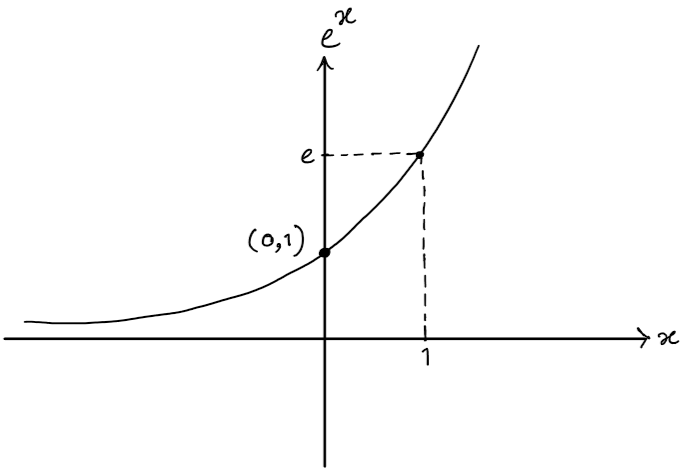
\includegraphics[scale=0.4]{images/fig13.png}
    \caption{La gráfica de la función exponencial.}
    \label{fig:fig13}
\end{figure}


\subsection{\col{Más acerca de la exponencial}}

Dado que ya se demostró que la función esponencial $\exp(x)$ es una función diferenciable y $\exp'(x)=\exp(x)$, se puede hacer la siguiente observación

$$ \integ[][]{\exp(x)}{dx}=\exp(x)+C.$$

Lo cual da lugar al siguinete teorema.

\begin{theorem}
    Si $f(x)$ es diferenciable, entonces 
    $$ \integ[][]{\exp(f(x))f'(x)}{dx}=\exp(f(x))+C.$$
\end{theorem}

\begin{proof}
    $$ {(\exp(f(x))+C)'}={(\exp(f(x)))'}=\exp(f(x))f'(x)$$
    $$\Rightarrow \quad \integ[][]{\exp(f(x))f'(x)}{dx}=\exp(f(x))+C. \quad $$
\end{proof}

Se demostrará que si $P(x)$ es cualquier polinomio en $x$, entonces $\lim_{x\to\infty}\frac{P(x)}{\exp(x)}=0$. Enseguida se mostrarán las ideas que ayudarán a llegar a esta conclusión.

\vspace{0.5cm}

Se probó que $\lim_{x\to\infty}\frac{x}{\exp(x)}=0$. Veamos que pasa con $\lim_{x\to\infty}\frac{x^2}{\exp(x)}$.

$$ \lim_{x\to\infty}\frac{x^2}{\exp(x)}=\lim_{x\to\infty}\frac{x^2}{\exp(\frac{x}{2}+\frac{x}{2})}=\lim_{x\to\infty}\frac{x^2}{\exp(\frac{x}{2})\exp(\frac{x}{2})}=\lim_{x\to\infty}\frac{x}{\exp(\frac{x}{2})}\frac{x}{\exp(\frac{x}{2})} $$
$$ =\lim_{x\to\infty}4\frac{\frac{x}{2}}{\exp(\frac{x}{2})}\frac{\frac{x}{2}}{\exp(\frac{x}{2})} $$

Sea $t=\frac{x}{2}$. Si $x\to \infty$, entonces $t\to \infty$, además, si $t\to \infty$, entonces $x\to \infty$, por lo tanto, $x\to \infty$, si y sólo si $t\to \infty$. De manera que

$$ \lim_{x\to\infty}4\frac{\frac{x}{2}}{\exp(\frac{x}{2})}\frac{\frac{x}{2}}{\exp(\frac{x}{2})}=\lim_{t\to\infty}4\frac{t}{\exp(t)}\frac{t}{\exp(t)}=2^2\lim_{x\to\infty}\frac{t}{\exp(t)}\lim_{x\to\infty}\frac{t}{\exp(t)}=2^2\cdot 0\cdot 0=0.$$

Ahora vease lo que ocurre con $\lim_{x\to\infty}\frac{x^3}{\exp(x)}$.

$$ \lim_{x\to\infty}\frac{x^3}{\exp(x)}=\lim_{x\to\infty}\frac{x^3}{\exp(\frac{x}{3}+\frac{x}{3})+\frac{x}{3}}=\lim_{x\to\infty}\frac{x^3}{\exp(\frac{x}{2})\exp(\frac{x}{2})\exp(\frac{x}{3})}$$
$$=\lim_{x\to\infty}\frac{x}{\exp(\frac{x}{3})}\frac{x}{\exp(\frac{x}{3})}\frac{x}{\exp(\frac{x}{3})}=\lim_{x\to\infty}27\frac{\frac{x}{3}}{\exp(\frac{x}{3})}\frac{\frac{x}{3}}{\exp(\frac{x}{3})}\frac{\frac{x}{3}}{\exp(\frac{x}{3})}.$$

Sea $t=\frac{x}{3}$. Si $x\to \infty$, entonces $t\to \infty$, además, si $t\to \infty$, entonces $x\to \infty$, por lo tanto, $x\to \infty$, si y sólo si $t\to \infty$. De manera que

$$ \lim_{x\to\infty}27\frac{\frac{x}{3}}{\exp(\frac{x}{3})}\frac{\frac{x}{3}}{\exp(\frac{x}{3})}\frac{\frac{x}{3}}{\exp(\frac{x}{3})}=\lim_{t\to\infty}27\frac{t}{\exp(t)}\frac{t}{\exp(t)}\frac{t}{\exp(t)}$$
$$=3^3\lim_{x\to\infty}\frac{t}{\exp(t)}\lim_{x\to\infty}\frac{t}{\exp(t)}\lim_{x\to\infty}\frac{t}{\exp(t)}=3^3\cdot 0\cdot 0=0.$$

\vspace{0.5cm}

En general, se cumple que si $k=\frac{x}{t}$, entonces $\lim_{x\to\infty}\frac{x^k}{\exp(x)}=\lim_{t\to\infty}k^k\left(\frac{t}{\exp(t)}\right)^k$. Con esto se puede probar el teorema pendiente.

\begin{theorem}
    Si $P(x)$ es cualquier polinomio en $x$, entonces 
    $$\lim_{x\to\infty}\frac{P(x)}{\exp(x)}=0.$$
\end{theorem}

\begin{proof}
    $$\limf{x}\frac{P(x)}{\exp(x)}=\limf{x}\frac{a_0+a_1x+a_2x^2+\cdots a_{n-1}x^{n-1}+a_nx^n}{\exp(x)}$$
    $$=\limf{x}\left( a_0\frac{1}{\exp(x)}+a_1\frac{x}{\exp(x)} a_2\frac{x^2}{\exp(x)}+\cdots+a_n\frac{x^n}{\exp(x)} \right)$$
    $$=\limf{x}\left( a_0\frac{1}{\exp(x)}+\suma{i=1}{n}{a_i(i)^{i}\left(\frac{\frac{x}{i}}{\exp(\frac{x}{i})}\right)^{i}} \right)=a_0(0)+a_1(0)+a_2(0)+\cdots+a_{n-1}(0)+a_n(0)=0$$
\end{proof}

\subsection{\col{Nueva notación para la exponencial}}

Se probará que $\exp(x)=e^x$. Esto se cumple en todos los casos, por ejemplo:

\begin{enumerate}
    \item[a)] $\exp(1)=e$.
    \item[b)] $\exp(2)=\exp(1+1)=\exp(1)\exp(1)=e\cdot e=e^2$.
    \item[c)] $\exp(n)=\exp(\underbrace{1+1+\cdots+1}_{\mbox{n veces}})=\underbrace{\exp(1)\exp(1)\cdots\exp(1)}_{\mbox{n veces}}=\exp(1)^n=e^n$.
    \item[d)] $\exp(-1)=\frac{1}{\exp(1)}=\exp(1)^{-1}=e^{-1}$.
    \item[e)] $\exp(-n)=\frac{1}{\exp(n)}=\frac{1}{e^n}=e^{-n}$.
\end{enumerate}

\begin{theorem}[(La constante de Euler)]
    $\exp(x)=e^{x}\quad\paratodoxen{x}{\mathbb{R}}$.
\end{theorem}

\begin{proof}
    $$ \exp(x)=\exp(\underbrace{1+1+\cdots+1}_{\mbox{$x$ veces}})=\underbrace{\exp(1)\exp(1)\cdots\exp(1)}_{\mbox{$x$ veces}}=\underbrace{e\cdot e\cdots e}_{\mbox{$x$ veces}}=e^x.$$
\end{proof}

\begin{theorem}
    $\exp(-x)=e^{-x} \quad \forall x\in\mathbb{R}$.
\end{theorem}

\begin{proof}
    $$ \exp(-x)=\frac{1}{\exp(x)}=\frac{1}{e^{x}}=(e^x)^{-1}=e^{-x}.$$
\end{proof}

\begin{theorem}
    $\left(\exp\left(\frac{1}{n}\right)\right)^m \paratodoxen{n,m}{R}$.
\end{theorem}

\begin{proof}
    $$ \left(\exp\left(\frac{1}{n}\right)\right)^m=\underbrace{\exp\left(\frac{1}{n}\right)\cdot\exp\left(\frac{1}{n}\right)\cdots\exp\left(\frac{1}{n}\right)}_{\mbox{$m$ veces}} $$
    $$ =\exp\left( \underbrace{\frac{1}{n}+\frac{1}{n}+\cdots+\frac{1}{n}}_{\mbox{$m$ veces}} \right)=\exp\left( m\left(\frac{1}{n}\right) \right)=\exp\left( \frac{m}{n} \right)=e^{\frac{m}{n}}.$$
\end{proof}

En conclusión, $\exp(x)=e^x \paratodoxen{x}{R}$.

\subsection{\col{Leyes de los exponentes}}

\begin{theorem}[Leyes de los exponentes]
    $\forall a,b\in\mathbb{R}$ y $\forall r\in\mathbb{Q}$ ocurre que:
    \begin{multicols}{3}
        \begin{enumerate}
            \item[a)] $e^a\cdot e^b=e^{a+b}$.
            \item[b)] $\frac{e^a}{e^b}=e^{a-b}$.
            \item[c)] $({e^a})^{r}=e^{ar}$.
        \end{enumerate}
    \end{multicols}
\end{theorem}

\begin{proof}
    \begin{enumerate}
        \item[a)] Por demostrar que $e^a\cdot e^b=e^{a+b}$.
        $$e^a\cdot e^b=\exp(a)\exp(b)=\exp(a+b)=e^{a+b}.$$
        \item[b)] Por demostrar que $\frac{e^a}{e^b}=e^{a-b}$.
        $$\frac{e^a}{e^b}=\frac{\exp(a)}{\exp(b)}=\exp(a-b)=e^{a-b}.$$
        \item[b)] Por demostrar que $({e^a})^{r}=e^{ar}$.
        $$({e^a})^{r}=e^{ar}=\exp(a)^{r}=\exp(ra)=\exp(ar)=e^{ar}.$$
    \end{enumerate}
\end{proof}

\subsection{\col{Cambio de base}}

Se observa que $x\ln(a)=\ln(a^x)$, entonces $\exp(x\ln(a))=\exp(\ln(a^x))=a^x$, pues la función exponencial es la inversa de la función logaritmo. Esta última igualdad da lugar a la siguiente definición:

\begin{definition}
    Sea $a>0$ una constante. Definimos 
    $$a^x=\exp(x\ln(a)).$$
\end{definition}

\textbf{Observación:} $1^x=\exp(x\ln(1))=\exp(x\cdot 0)=\exp(0)=1 \quad \paratodoxen{x}{R}$.

\vspace{0.5cm}

Sea $a>0$, entonces la función $f(x)=a^x$ es diferenciable y $\derivate{x}{f(x)}=\derivate{x}{a^x}=\derivate{x}{\exp(x\ln(a))}=\exp(x\ln(a))\derivate{x}{(x\ln(a))}=\exp(x\ln(a))(\ln(a))=a^x\ln(a)$. De lo que podemos concluir que, si $f(x)=a^x$, entonces $\derivate{x}{f(x)}=a^x\ln(a)$.

\begin{theorem}
    Sea $a>0$ y $a\neq 1$, entonces $\integ[][]{a^x}{dx}=\frac{a^x}{\ln(a)}+C$.
\end{theorem}

\begin{proof}
    Se observó que si $f(x)=a^x$, entonces $\derivate{x}{f(x)}=a^x\ln(a)$, por lo tanto $\integ[][]{a^x\ln(a)}{dx}=a^x+C$, de manera que $\ln(a)\integ[][]{a^x}{dx}=a^x+C$, se sigue que 
    $$\integ[][]{a^x}{dx}=\frac{a^x}{\ln(a)}+\frac{C}{\ln(a)}=\frac{a^x}{\ln(a)}+C'.$$  
\end{proof}


\subsection{\col{La gráfica de la función \ensuremath{a^x} con \ensuremath{a} fijo}}

A continuación se trazará con todo detalle la gráfica de la función $f(x)=a^x$ enunciando todas sus propiedades: 0) Dominio, imagen y puntos por los que pasa la función; 1) Primera derivada, intervalos de crecimiento y decrecimiento, y puntos críticos estacionarios o puntos singulares; 2) Segunda derivada, intervalos de concavidad positiva y negativa, y puntos de inflexión; 3) Límites relevantes y comportamiento asintótico. 

\begin{enumerate}
    \item[0)] $Dom(a^x)=(-\infty,\infty)$, $Im(a^x)=(0,\infty)$ y Pasa por los puntos $(0,1)$ y $(1,a)$.
    \item[1)] $$ \derivate{x}{a^x}=a^x\ln(a)
    \left\{
        \begin{array}{lll}
            <0  & \mbox{si } 0<a<1 \\
            \\ =0 & \mbox{si } a=1 \\
            \\ >0 & \mbox{si } 1<a \\
        \end{array}
    \right.$$
    
    Por lo tanto:
    
    \begin{enumerate}
    
    \item[\textbf{Caso 1.}]  $0<a<1$
    \begin{enumerate}
    \item Intervalo de crecimiento$=\varnothing$.
    \item Intervalo de decrecimiento$=(-\infty,\infty)$.
    \item No existen puntos críticos estacionarios.
    \end{enumerate} 
    
    \item[\textbf{Caso 2.}]  $a=1$
    \begin{enumerate}
    \item Intervalo de crecimiento$=\varnothing$.
    \item Intervalo de decrecimiento$=\varnothing$.
    \item No existen puntos críticos estacionarios.
    \end{enumerate} 
    
    \item[\textbf{Caso 3.}]  $1<a$
    \begin{enumerate}
    \item Intervalo de crecimiento$=(-\infty,\infty)$.
    \item Intervalo de decrecimiento$=\varnothing$.
    \item No existen puntos críticos estacionarios.
    \end{enumerate} 
    
    \end{enumerate}
    
    \item[2)] $$ \frac{\mathrm{d^2}}{\mathrm{d}x} \left(  {a^x}  \right)  
    \left\{
        \begin{array}{ll}
            >0  & \mbox{si } a\neq 1 \\
            \\ =0 & \mbox{si } a=1 \\
        \end{array}
    \right.$$
    
    Por lo tanto:
    
    \begin{enumerate}
    
    \item[\textbf{Caso 1.}]  $0<a<1$
    \begin{enumerate}
    \item Intervalo de concavidad positiva$=(-\infty,\infty)$.
    \item Intervalo de concavidad negativa$=\varnothing$.
    \item No existen puntos de inflexión.
    \end{enumerate} 
    
    \item[\textbf{Caso 2.}]  $a=1$
    \begin{enumerate}
    \item Intervalo de concavidad positiva$=\varnothing$.
    \item Intervalo de concavidad negativa$=\varnothing$.
    \item No existen puntos de inflexión.
    \end{enumerate} 
    
    \item[\textbf{Caso 3.}]  $1<a$
    \begin{enumerate}
    \item Intervalo de concavidad positiva$=(-\infty,\infty)$.
    \item Intervalo de concavidad negativa$=\varnothing$.
    \item No existen puntos de inflexión.
    \end{enumerate} 
    
    \end{enumerate}
    
    \item[3)] Límites relevantes 
    
    \begin{enumerate}
    
    \item[\textbf{Caso 1.}]  $0<a<1$
    \begin{enumerate}
    \item $\limf{x}a^x=\limf{x}\exp(x\ln(a))=0$.
    \item $\limit{x}{-\infty}a^x=\limit{x}{-\infty}\exp(x\ln(a))=\infty$.
    \end{enumerate} 
    
    \item[\textbf{Caso 2.}]  $a=1$
    \begin{enumerate}
    \item $\limf{x}a^x=\limf{x}\exp(x\ln(a))=\limf{x}\exp(x\cdot 0)=1$.
    \item $\limit{x}{-\infty}a^x=\limit{x}{-\infty}\exp(x\ln(a))=\limit{x}{-\infty}\exp(x\cdot 0)=1$.
    \end{enumerate} 
    
    \item[\textbf{Caso 3.}]  $1<a$
    \begin{enumerate}
    \item $\limf{x}a^x=\limf{x}\exp(x\ln(a))=\infty$.
    \item $\limit{x}{-\infty}a^x=\limit{x}{-\infty}\exp(x\ln(a))=0$.
    \end{enumerate} 
    
    \end{enumerate}
    
\end{enumerate}

\vspace{0.5cm}

Dado lo anterior, la gráfica de la función $f(x)=a^x$ tiene el siguiente aspecto:

\begin{figure}[H]
    \centering
    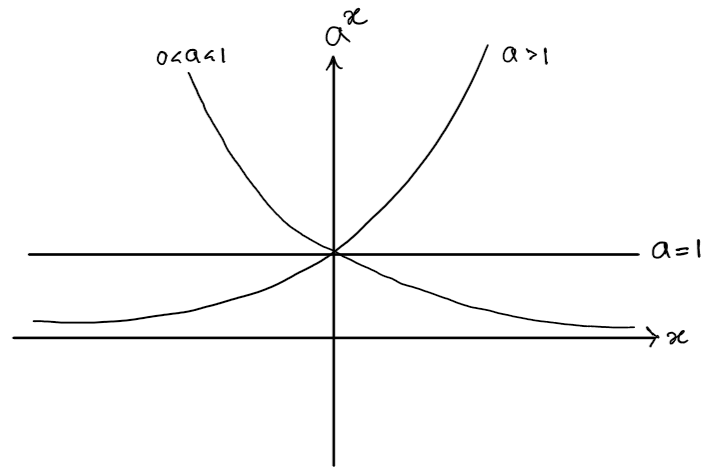
\includegraphics[scale=0.4]{images/fig14.png}
    \caption{La gráfica de la función $a^x$.}
    \label{fig:fig14                                                    }
\end{figure}

\begin{theorem}
    Si $1<a<b$, entonces 
    \begin{enumerate}
        \item[a)] $a^x<b^x$ si $x>0$.
        \item[b)] $a^x=b^x$ si $x=0$.
        \item[c)] $a^x>b^x$ si $x<0$.
    \end{enumerate}
\end{theorem}

\begin{proof}
    Sea $\frac{a^x}{b^x}=\frac{\exp(x\ln(a))}{\exp(x\ln(b))}=\exp(x\ln(a))\cdot\exp(x\ln(b))^{-1}=\exp(x\ln(a))\cdot\exp(-x\ln(b))=\exp(x\ln(a)-x\ln(b))=\exp(x(\ln(a)-\ln(b)))$, entonces $\frac{a^x}{b^x}=\exp(x[\ln(a)-\ln(b)])$. 
    Si $r=\ln(a)-\ln(b)$, entonces $r<0$ y 

    $$\frac{a^x}{b^x}=\exp(x\cdot r)
    \left\{
        \begin{array}{lll}
            <1  & \mbox{si } x>0 & \mbox{, entonces} \quad a^x<b^x \\
            \\ =1 & \mbox{si } x=0 & \mbox{, entonces} \quad a^x=b^x \\
            \\ >1 & \mbox{si } x<0 & \mbox{, entonces} \quad a^x>b^x \\
        \end{array}
    \right.$$
\end{proof}

\begin{theorem}
    Si $0<a<b<1$, entonces
\begin{enumerate}
\item[i)] $a^x<b^x$ si $x>0$.
\item[ii)] $a^x=b^x$ si $x=0$. 
\item[iii)] $a^x>b^x$ si $x<0$.
\end{enumerate}
\end{theorem}


\begin{proof}
    Sea $\frac{a^x}{b^x}=\exp(x[\ln(a)-\ln(b)])$. Si $r=\ln(a)-\ln(b)$, entonces $r<0$ y

$$ \frac{a^x}{b^x}=\exp(r\cdot x)\left\{
    \begin{array}{lll}
        <1  & \mbox{si } x>0 & \mbox{, entonces} \quad a^x<b^x \\
        \\ =1 & \mbox{si } x=0 & \mbox{, entonces} \quad a^x=b^x \\
        \\ >1 & \mbox{si } x<0 & \mbox{, entonces} \quad a^x>b^x. \\
    \end{array}
\right.$$
\end{proof}

En resumen, se definió la función $f(x)=a^x=\exp(x\ln(a))$ con $a>0$ constante, se estudio el caso especial $a=1$ y se demostró el aspecto del siguiente gráfico:

\begin{figure}[H]
    \centering
    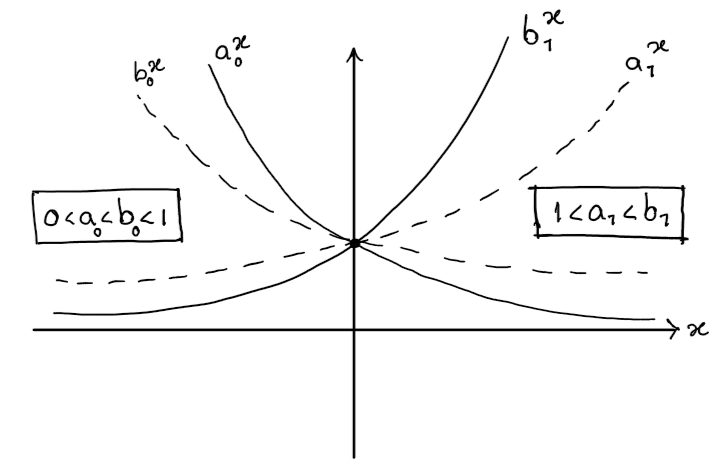
\includegraphics[scale=0.4]{images/fig15.png}
    \caption{\textbf{Nota:} $a_0$, $b_0$, $a_1$ y $b_1$ constantes.}
    \label{fig:fig14                                                    }
\end{figure}

\subsection{\col{Algunas propiedades algebraicas}}

\begin{theorem}
    Sea $a$ constante, entonces
\begin{enumerate}
\item[i)] $a^xa^y=a^{x+y}$.
\item[ii)] $a^{-x}=\frac{1}{a^{-x}}$.
\item[iii)] $\frac{a^x}{a^y}=a^{x-y}$.
\item[iv)] $\left(a^x\right)^y=a^{xy}$.
\end{enumerate}
\end{theorem}

\begin{proof}
    \begin{enumerate}
        \item[i)] Por demostrar $a^xa^y=a^{x+y}$.
        
        \begin{equation*}
        \begin{split}
            a^xa^y & =\exp(x\ln(a))\cdot\exp(y\ln(a))=\exp(x\ln(a)+y\ln(a))=\exp(\ln(a)(x+y))\\
            & =\exp(\ln(a^{x+y}))=a^{x+y}.
        \end{split}
        \end{equation*}
        
        \item[ii)] Por demostrar  $a^{-x}=\frac{1}{a^{-x}}$.
        
        \begin{equation*}
        \begin{split}
            a^{-x} & =\exp(-x\ln(a))=\exp(x\ln(a))^{-1}=\frac{1}{\exp(\ln(a^x))}=\frac{1}{a^x}.
        \end{split}
        \end{equation*}
        
        \item[iii)] Por demostrar $\frac{a^x}{a^y}=a^{x-y}$.
        
        \begin{equation*}
        \begin{split}
            \frac{a^x}{a^y} & =\frac{\exp(x\ln(a))}{\exp(y\ln(a)}=\exp(x\ln(a))\cdot\exp(y\ln(a))^{-1}=\exp(x\ln(a))\cdot\exp(-y\ln(a)) \\
            & =\exp(x\ln(a)-y\ln(a))=\exp(\ln(a)(x-y))=\exp(\ln(a^{x-y})) \\
            & =a^{x-y}.
        \end{split}
        \end{equation*}
        
        \item[iv)] Por demostrar $\left(a^x\right)^y=a^{xy}$.
        
        \begin{equation*}
        \begin{split}
            \left( a^x \right)^y &=\exp(x\ln(a))^y=\exp(xy\ln(a))=\exp(\ln(a^{xy}))=a^{xy}.  \\
        \end{split}
        \end{equation*}
        
        \end{enumerate}
\end{proof}

\begin{theorem}
    $ \limit{n}{\infty} n\left( \sqrt[n]{x}-1 \right)=\ln(x) $.
\end{theorem}

\begin{proof}
    $$\limit{n}{\infty} n\left(\sqrt[n]{x}-1\right)=\limit{n}{\infty}\frac{x^{\frac{1}{n}}-1}{\frac{1}{n}}.$$
    Sea $b=\frac{1}{n}$, entonces 
    $$\limit{b}{0}\frac{x^b-1}{b}=\limit{b}{0}\frac{x^b-x^0}{b}=\limit{b}{0}\frac{\exp(b\ln(x))-\exp(0\ln(x))}{b}.$$
    Además, $\limit{b}{0}\frac{\exp(b\ln(x)) -\exp(0\ln(x))}{b}=\limit{b}{0}\frac{f(b)-f(0)}{b}=f'(0)$ donde $f(b)=\exp(b\ln(x))$. Entonces 
    $$\limit{n}{\infty} n\left( \sqrt[n]{x}-1  \right)=f'(0)=\ln(x)$$.
\end{proof}

\subsection{\col{Arsenal de límites hasta este punto}}

\begin{multicols}{2}
    \begin{enumerate}
        \item $\limf{x}\ln(x)=\infty$
        \item $\limit{x}{0^+}\ln(x)=-\infty$
        \item $\limit{x}{\infty}\frac{\ln(x)}{x}=0$
        \item $\limit{x}{\infty}\frac{\ln(x)}{ax+b}=0$
        \item $\limit{x}{0^+}\frac{\ln(x)}{x}=-\infty$
        \item $\limit{x}{0^+}x\ln(x)=0$
        \item $\limit{x}{\infty}\frac{1+x^2}{x}=0$
        \item $\limit{x}{\infty}\exp(x)=\infty$
        \item $\limit{x}{-\infty}\exp(x)=0$
        \item $\limit{x}{\infty}\frac{x}{\exp(x)}=0$
        \item $\limit{x}{\infty}\frac{ax+b}{\exp(x)}=0$
        \item $\limit{x}{1}\frac{\ln(t)}{t-1}=1$
        \item $\limit{x}{0}\frac{\exp(x)-1}{x}=1$
        \item $\limit{x}{\infty}\frac{p(x)}{\exp(x)}=0$
        \item $\limit{x}{\infty}\frac{x^k}{\exp(x)}=0$
        \item $\limit{x}{0^+}x^x=1$
        \item $\limit{x}{\infty}x^{\frac{1}{x}}=1$
        \item $\limit{n}{\infty}n(x^{\frac{1}{n}}-1)=\ln(x)$
    \end{enumerate}
\end{multicols}

\subsection{\col{Ejercicios}}

\begin{enumerate}
    \item Simplifique lo siguiente:
    \begin{multicols}{3}
        \begin{enumerate}
            \item[a)] $\ln{(\exp(x-\ln(x)))}$
            \item[b)] $\exp(-\ln(x))$
            \item[c)] $\exp(-\ln(\exp(2x^2+1)))$
        \end{enumerate}
    \end{multicols}
    \item Calcule la primera derivada de las siguientes funciones:
    \begin{multicols}{2}
        \begin{enumerate}
            \item[a)] $f(x)=\exp(\sen(x))$
            \item[c)] $h(x)=x\exp(-x^3)$
            \item[b)] $g(x)=\exp\left(\frac{1}{\ln(x)}\right)$
            \item[d)] $k(x)=\ln(\exp(x)+\exp(-x))$
        \end{enumerate}
    \end{multicols}
    \item Resuelva los siguiente: 
    \begin{multicols}{2}
        \begin{enumerate}
            \item[a)] $\integrate{}{}{\exp(\sen(x))\cos(x)}{x}$
            \item[c)] $\integrate{}{}{\exp(\exp(x)+x)[\exp(x)+1]}{x}$
            \item[b)] $\integrate{}{}{\frac{\exp(x^{-1})}{x^2}}{x}$
        \end{enumerate}
    \end{multicols}
    \item Trace la gráfica de $f(x)=exp(-x)$.
    \item Calcule lo siguiente:
    \begin{multicols}{2}
        \begin{enumerate}
            \item[a)] $\der{x}10^x$
            \item[b)] $\der{x}e^x$
        \end{enumerate}
    \end{multicols}
    \item Trace la gráfica de $f(x)=x^x$.
    \item Demuestre que si $0<x<1$, entonces $\frac{x-1}{x}\leq\ln(x)\leq x-1$.
    \item Tace la gráfica de $f(x)=x^{\frac{1}{2}}$.
    \item Calcule lo siguiente:
    \begin{multicols}{3}
        \begin{enumerate}
            \item[a)] $\integrate{0}{1}{2^{-x}}{x}$
            \item[b)] $\integrate{0}{\pi /2}{7^{\cos(\theta)}3\sen(\theta)}{\theta}$
            \item[c)] $\integrate{-\ln(3)}{\ln(4)}{x(3^{x^2})}{x}$
        \end{enumerate}
    \end{multicols}
\end{enumerate}

\subsection{\col{Logaritmo base \ensuremath{a} de \ensuremath{x}}}

Se vio que $e^x=\exp(x)$ y que $a^x=\exp(x\ln(a))$, ahora se hablará de $\log_a(x)$. Pues el contenido anterior trató de $\ln(x)=\log_e(x)$. Se sabe que la función $f(x)=a^x$ tiene el siguiente aspecto para diferentes valores de $a$ tal que $a\in(0,1)\cup(1,\infty)$:

\begin{figure}[H]
    \centering
    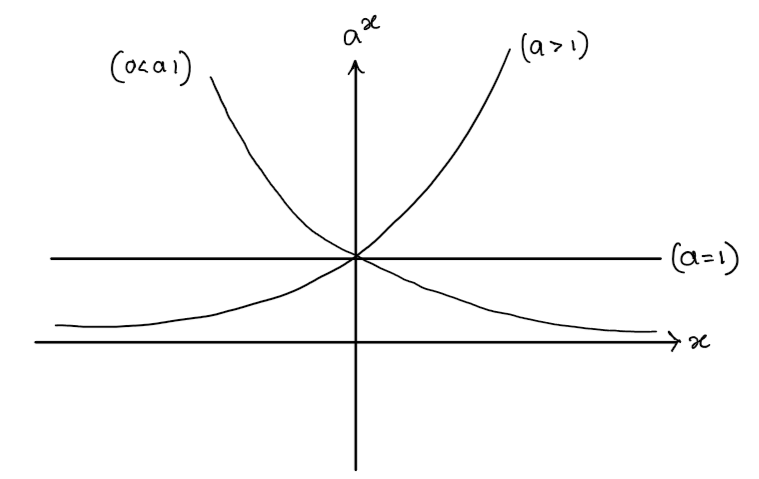
\includegraphics[scale=0.4]{images/fig16.png}
    \caption{\textbf{Nota:} $a$ constante.}
    \label{fig:fig16}
\end{figure}

Para encontrar $\log_a(x)$ habrá que invertir $a^x \quad \forall x\in (0,1)\cup (1,\infty)$. Sea $a>0$ ($a\neq 1$). Se probó que $a^x:(-\infty,\infty)\to (0,\infty)$ es una función biyectiva por lo tanto es invertible.

\begin{definition}[(Logaritmo base $a$ de $x$)]
    $\log_a(x):\left(0,\infty\right)\to\left(-\infty,\infty\right)$ se define como la función inversa de $a^x$, tal que $x=\log_a(y)$ si y sólo si $y=a^x$, de manera que $x=\log_a(a^x)$.
\end{definition}

En particular, sucede que $a^{\log_a(x)}=x$, por lo que podemos decir que "el logaritmo base $a$ de $x$ es el exponente al cual hay que elevar $a$ para obtener $x$". Como $\log_{a}(x)$ es la función inversa de $a^x$, entonces se tiene que

$$ \log_a(a^x)=x=a^{\log_a(x)}. $$

Por definición, $a^{\log_a(x)}=x$, entonces, aplicando logaritmo natural en ambos lados de la desigualdad se obtiene que $\ln(a^{\log_a(x)})=\ln(x)$, por lo que $\log_a(x)\ln(a)=\ln(x)$, de modo que, despejando, se obtiene un manera sencilla de calcular $\log_a(x)$: 
$$\log_a(x)=\frac{1}{\ln(a)}\ln(x).$$ 

\vspace{0.5cm}

\textbf{Observación:} Como $\ln(e)=1$, entonces se tiene que
$$ \log_e(x)=\frac{1}{\ln(e)}\ln(x)=\ln(x).$$

\subsection{\col{Propiedades del logaritmo base \ensuremath{a}}}

\begin{theorem}[(Propiedades del logaritmo base $a$)]
    Sean $x,y>0$ y $r\in\mathbb{R}$, entonces 
    \setlength{\columnsep}{-1.1in}
\begin{multicols}{2}
    \begin{itemize}
        \item[i)] $\log_a(xy)=\log_a(x)+\log_a(y)$,
        \item[ii)] $\log_a(x^{-1})=-\log_a(x)$,
        \item[iii)] $\log_a(\frac{x}{y})=\log_a(x)-\log_a(y)$,
        \item[iv)] $\log_a(x^r)=r\log_a(x)$.
    \end{itemize}
\end{multicols}
\end{theorem}

\begin{proof}
    La demostración del teorema se realizará utilizando la definición de logaritmo natural base $a$ y las propiedades del logaritmo natural anteriormente demostradas. 
    \begin{enumerate}

        \item[i)]
        $$\begin{aligned}
            \log_a(xy) & = \frac{1}{\ln(a)}\ln(xy)=\frac{1}{\ln(a)}\left[ \ln(x)+\ln(y) \right]=\frac{1}{\ln(a)}\ln(x)+\frac{1}{\ln(a)}\ln(y) \\
            &  =\log_a(x)+\log_a(y). \\
        \end{aligned}$$
        
        \item[ii)]
        $$ \log_a(x^{-1})=\frac{1}{\ln(a)}\ln(x^{-1})=-\frac{1}{\ln(a)}\ln(x)=-\log_a(x). $$
        
        \item[iii)]
        \begin{equation*}
        \begin{split}
        \log_a\left(\frac{x}{y}\right) & =\frac{1}{\ln(a)}\log\left(\frac{x}{y}\right)=\frac{1}{\ln(a)}\left[ \ln(x)-\ln(y) \right] \\ 
        & =\frac{1}{\ln(a)}\ln(x)-\frac{1}{\ln(a)}\ln(y)=\log_a(x)-\log_a(y).
        \end{split}
        \end{equation*}
        
        \item[iv)]
        $$ \log_a\left(x^r\right)=\frac{r}{\ln(a)}\ln(x)=r\log_a(x). $$
        
        \end{enumerate}
\end{proof}

\subsection{\col{Límites relevantes para \ensuremath{\log_a(x)} }}

\begin{theorem}
    Sea $a\in\mathbb{R}$ tal que $a>0$, entonces 
    \setlength{\columnsep}{-0.6in}
    \begin{multicols}{2}
        \begin{itemize}
            \item[i)] $\limit{x}{\infty}\log_a(x)=\infty\quad$ si $\quad a>1$.
            \item[ii)] $\limit{x}{\infty}\log_a(x)=-\infty\quad$ si $\quad 0<a<1$.
            \item[iii)] $\limit{x}{0^+}\log_a(x)=-\infty\quad$ si $\quad a>1$.
            \item[iv)] $\limit{x}{0^+}\log_a(x)=\infty\quad$ si $\quad 0<a<1$.
        \end{itemize}
    \end{multicols}
\end{theorem}

\begin{proof}
    \begin{enumerate}
        \item[i)] Si $a>1$, entonces $\frac{1}{\ln(a)}>0$ de manera que 
        $$ \limit{x}{\infty}\log_a(x)=\limit{x}{\infty}\frac{1}{\ln(a)}\ln(x)=\frac{1}{\ln(a)}\limit{x}{\infty}\ln(x)=\infty. $$
        \item[ii)] Si $0<a<1$, entonces $\frac{1}{\ln(a)}<0$ de modo que 
        $$ \limit{x}{\infty}\log_a(x)=\limit{x}{\infty}\frac{1}{\ln(a)}\ln(x)=\frac{1}{\ln(a)}\limit{x}{\infty}\ln(x)=-\infty. $$
        \item[iii)] Si $a>1$, entonces $\frac{1}{\ln(a)}>0$ de manera que 
        $$ \limit{x}{0^+}\log_a(x)=\limit{x}{0^+}\frac{1}{\ln(a)}\ln(x)=\frac{1}{\ln(a)}\limit{x}{0^+}\ln(x)=-\infty .$$
        \item[iv)] Si $0<a<1$, entonces $\frac{1}{\ln(a)}<0$ de modo que 
        $$ \limit{x}{0^+}\log_a(x)=\limit{x}{0^+}\frac{1}{\ln(a)}\ln(x)=\frac{1}{\ln(a)}\limit{x}{0^+}\ln(x)=\infty .$$
        \end{enumerate}
\end{proof}

\subsection{\col{La gráfica de la función \ensuremath{\log_a(x)} con \ensuremath{a} fijo}}

A continuación se examinaran las propiedades de la función $f(x)=\log_a(x)$ para hallar esbozar su gráfica.

% \begin{multicols}{2}
%     \begin{enumerate}
%         \setcounter{enumi}{0}
%         \item Dominio e imagen
%         \item Imagen de puntos por los que pasa la \\ función.
%         \item Primera derivada
%         \item Intervalos de crecimiento \\ y decredimiento
%         \item Puntos críticos estacionarios o \\ singulares
%         \item Segunda de derivada
%         \item Intervalos de concavidad positiva y negativa
%         \item Puntos de inflexión
%         \item Limites relevantes
%         \item Comportamiento asintótico 
%     \end{enumerate}
% \end{multicols}

\subsubsection{Dominio e imagen}
$$Dom\left( \log_a(x) \right)=(0,\infty) \quad\quad\quad Img\left(\log_a(x)\right)=(-\infty,\infty)$$

\subsubsection{Imagen de puntos por los que pasa la función}

Pasa por $(1,0)$.

\subsubsection{Primera derivada}

$$\der{x}f(x)=\frac{1}{\ln(a)x}
\left\{
    \begin{array}{ll}
        >0  & \mbox{si } 1<a \\
        <0 & \mbox{si } 0<a<1 \\
    \end{array}
\right.$$

Entonces la función es creciente en el intervalo $(0,\infty)$ cuando $1<a$ y decreciente en el intervalo $(0,\infty)$ cuando $0<a<1$.

\subsubsection{Segunda derivada}
$$\derivada{2}{x^2}f(x)=-\frac{1}{\ln(a)x^2}
\left\{
\begin{array}{ll}
    >0 & \mbox{si } 0<a<1 \\
    <0 & \mbox{si } 1<a
\end{array}
\right.$$

Entonces la función tiene concavidad positica en el inertvalo $(0,\infty)$ cuando $0<a<1$ y tiene concavidad negativa en el intervalo $(0,\infty)$. En ningún caso se observan puntos de inflexión.

\subsubsection{Comportamiento límite}

$$
\limf{x}\log_a(x)=\left\{
\begin{array}{ll}
    \infty & \mbox{si } 1<a \\
    -\infty & \mbox{si } 0<a<1
\end{array}    
\right. 
\quad\quad 
\limit{x}{o^+} \log_a(x)=\left\{
\begin{array}{ll}
    -\infty & \mbox{si } 1<a \\
    \infty & \mbox{si } 0<a<1
\end{array}    
\right. 
$$

\subsubsection{Gráfica de la función}

Entonces la función tiene el siguiente aspecto:

\begin{figure}[H]
    \centering
    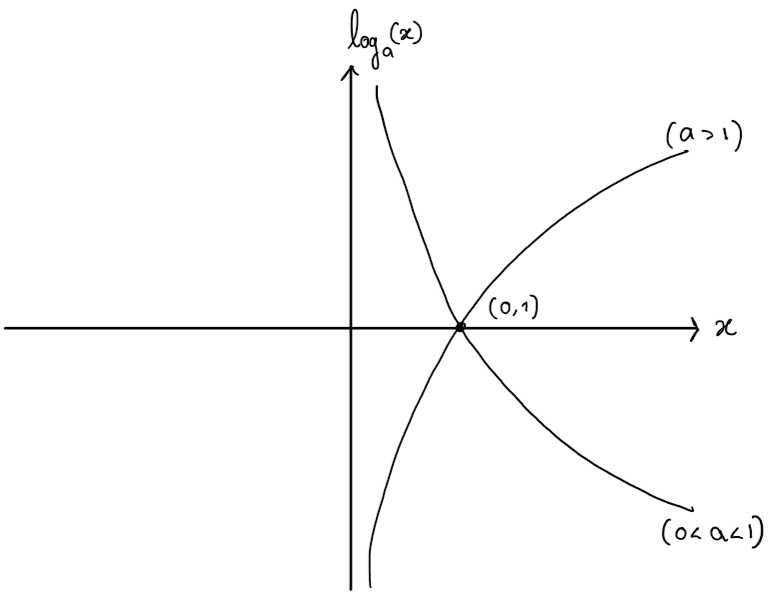
\includegraphics[scale=0.4]{images/fig17.png}
    \caption{\textbf{Nota:} $a$ constante.}
    \label{fig:fig17}
\end{figure}

Se obervan los siguientes 4 casos:
\begin{itemize}
\item Si $1<a<b$ y $x>1$, entonces $$\log_a(x)=\frac{1}{\ln(a)}\ln(x)\geq \frac{1}{\ln(b)}\ln(x)=log_b(x).$$
\item Si $1<a<b$ y $0<x<1$, entonces $$\log_a(x)=\frac{1}{\ln(a)}\ln(x)\leq \frac{1}{\ln(b)}\ln(x)=log_b(x).$$
\item Si $0<a<b<1$ y $x>1$, entonces $$\log_a(x)=\frac{1}{\ln(a)}\ln(x)> \frac{1}{\ln(b)}\ln(x)=log_b(x).$$
\item Si $0<a<b<1$ y $0<x<1$, entonces $$\log_a(x)=\frac{1}{\ln(a)}\ln(x)< \frac{1}{\ln(b)}\ln(x)=log_b(x).$$    
\end{itemize}

Entonces se puede demostrar el aspecto del siguiente gráfico:

\begin{figure}[H]
    \centering
    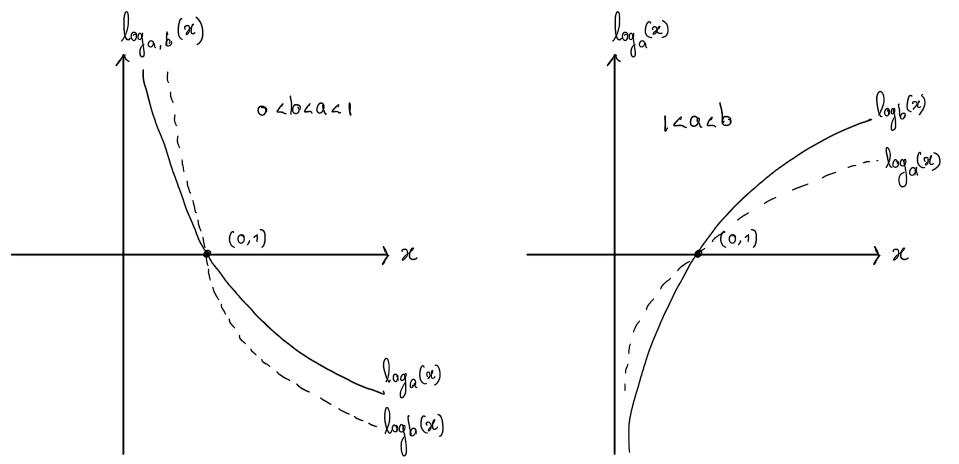
\includegraphics[scale=0.5]{images/fig18.png}
    \caption{\textbf{Nota:} $a$ y $b$ constantes.}
    \label{fig:fig18}
\end{figure}

\begin{theorem}
    Para $x>0$ se tiene que
$$ \int\!\ln(x)\mbox{ d}x=x\ln(x)-x+C.$$
\end{theorem}

\begin{proof}
    $$\begin{aligned}
        \der{x}\left\{x\ln(x)-x+C\right\} & = \der{x}\left\{x\ln(x)\right\} -1  \\
        & = \ln(x)+x\frac{1}{x}-1 \\ 
        & = \ln(x) \\ 
    \end{aligned}$$
    
    Por lo tanto se tiene que
    
    $$x\ln(x)-x+C=\int\!\der{x}\left\{x\ln(x)-x+C\right\}\mbox{ d}x=\int\!\ln(x)\mbox{ d}x.$$
        
\end{proof}

\subsection{\col{Cambio de base}}

Se hallará la respuesta a preguntas similares a la siguiente: ¿Cuánto es $\log_a(x)$ si se conoce el valor de $\log_b(x)$ y $a\neq b$ con $a\neq 1$ y $b\neq 1$? Se sabe que 

$$\log_a(x)=\frac{\ln(x)}{\ln(a)} \quad \mbox{y} \quad \log_b(x)=\frac{\ln(x)}{\ln(b)},$$
$$\Leftrightarrow \quad \ln(x)=\log_a(x)\ln(a) \quad \mbox{y} \quad \ln(x)=\log_b(x)\ln(b), $$
$$\Leftrightarrow \quad \log_a(x)\ln(a)=\log_b(x)\ln(b).$$

Por lo tanto

$$\log_a(x)= \frac{\ln(b)}{\ln(a)}\log_b(x).$$

En este caso, el cociente $\frac{\ln(b)}{\ln(a)}$ es el factor de cambio de base.

\subsection{\col{Ejercicios}}
\begin{enumerate}
    \item Calcule lo siguiente:
    \begin{multicols}{3}
        \begin{enumerate}
            \item[a)] $\integrate{}{}{\frac{\log_a(x)}{x}}{x}$ 
            \item[b)] $\integrate{}{}{\frac{1}{x\log_a(x)}}{x}$ 
            \item[c)] $\integrate{}{}{\log_a(x)}{x}$ 
        \end{enumerate}
    \end{multicols}
    \item Demuestre que $$\integrate{}{}{\ln(x)}{x}=x\ln(x)-x+c$$ con $c$ una constante.
    \item ¿Cuánto es $\log_2(x)$ si $\log_3(x)=9$?
\end{enumerate}

\newpage

\section{\col{Funciones hiperbólicas}}

\begin{definition}[(Seno y coseno hiperbólico)]
    El seno hiperbólico es una función $senh:\mathbb{R}\rightarrow\mathbb{R}$ tal que 
$$senh(x)=\frac{e^x-e^{-x}}{2}\quad\quad\forall x\in\mathbb{R},$$
y el coseno hiperbólico es una función $cosh:\mathbb{R}\rightarrow\mathbb{R}$ tal que 
$$cosh(x)=\frac{e^x+e^{-x}}{2}\quad\quad\forall x\in\mathbb{R}.$$
\end{definition}

A partir de las definiciones anteriores de pueden definir el resto de las funciones hiperbólicas.
$$\begin{array}{lll}
    \tanh:\mathbb{R}\rightarrow\mathbb{R}\quad\quad\quad & \tanh(x)=\frac{\senh(x)}{\cosh(x)}=\frac{e^x-e^{-x}}{e^x+e^{-x}}\quad\quad\quad & \forall x\in\mathbb{R} \\
    \\
    \coth:\mathbb{R}\rightarrow\mathbb{R}\quad\quad\quad & \coth(x)=\frac{\cosh(x)}{\senh(x)}=\frac{e^x+e^{-x}}{e^x-e^{-x}}\quad\quad\quad & \forall x\in\mathbb{R} \\
    \\
    \sech:\mathbb{R}\rightarrow\mathbb{R}\quad\quad\quad & \sech(x)=\frac{1}{\cosh(x)}=\frac{2}{e^x+e^{-x}}\quad\quad\quad & \forall x\in\mathbb{R} \\
    \\
    \csch:\mathbb{R}\rightarrow\mathbb{R}\quad\quad\quad & \csch(x)=\frac{1}{\senh(x)}=\frac{2}{e^x-e^{-x}}\quad\quad\quad & \forall x\in\mathbb{R} \\
\end{array}$$

Su motivacion es simple:

\begin{multicols}{2}
    Si $C=\{(u,v)\in\mathbb{R}^2 | u^2+v^2=1\}$, entonces $P=(\cos(x), \sen(x))\in C$
    \begin{figure}[H]
        \centering
        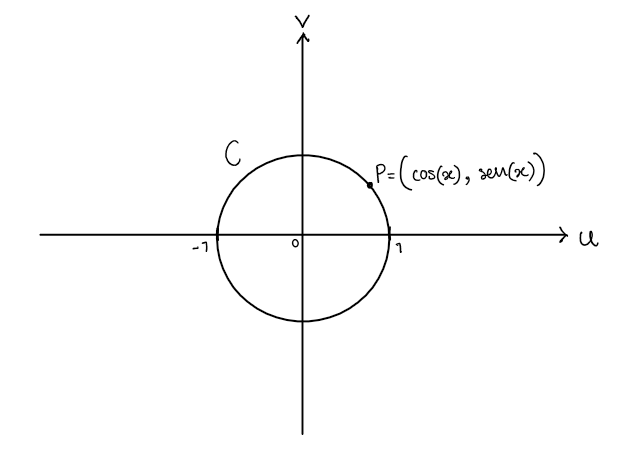
\includegraphics[scale=0.4]{images/fig19.png}
        \label{fig:fig19}
    \end{figure}
    Si $H=\{(u,v)\in\mathbb{R}^2 | u^2-v^2=1\}$, entonces $P=(\cosh(x), \senh(x))\in H$
    \begin{figure}[H]
        \centering
        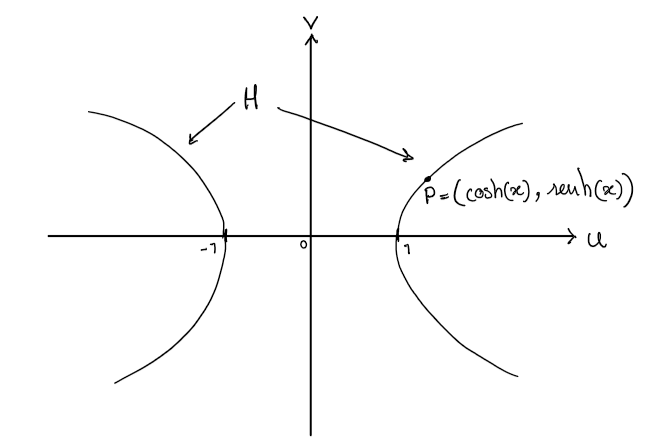
\includegraphics[scale=0.4]{images/fig20.png}
        \label{fig:fig20}
    \end{figure}
\end{multicols}

Las analogias entre el mundo trigonométrico y el mundo hiperbólico son diversas. A continuación se muestran algunas propiedades.

\hspace{1cm}

\begin{center}
{\tabulinesep=1.2mm
\begin{tabu} {|c|c|}
    \hline
    \textbf{Mundo hiperbólico} &  \textbf{Mundo trigonométrico} \\ 
    \hline
    $\der{x}\senh(x)=\cosh(x)$ & $\der{x}\sen(x)=\cos(x)$ \\
    \hline
    $\der{x}\cosh(x)=\senh(x)$ & $\der{x}\cos(x)=\sen(x)$ \\ [0.5ex]
    \hline
    $\cosh(x)^2-\senh(x)^2=1$ & $\cosh(x)^2+\senh(x)^2=1$ \\
    \hline
$\senh(x\pm y)=\senh(x)\cosh(y)\pm \senh(y)\cosh(x)$ & $\begin{array}{c}
    \sen(x\pm y)=\cos(x)\sen(y)\pm \cos(y)\sen(x) \\ 
    \cos(x\pm y)=\cos(x)\cos(y)\mp \sen(y)\sen(x) \\
\end{array}$ \\
    \hline
    Ley de De Moivre & \\
    $\left(\cosh(x)+\senh(x)\right)^2=\cosh(nx)+\senh(nx)$ & $\left(\cos(x)+i\sen(x)\right)^2=\cos(nx)+i\sen(nx)$ \\
    \hline
\end{tabu}}
\end{center}

\begin{theorem}
	$\senh'(x)=cosh(x)$
\end{theorem}

\begin{proof}
	$$\senh'(x)=\der x \senh(x)=\der x \frac{e^x-e^{-x}}{2}=\frac{e^x+e^{-x}}{2}=\cosh(x)$$
\end{proof}

\begin{theorem}
	$\cosh'(x)=senh(x)$
\end{theorem}

\begin{proof}
	$$\cosh'(x)=\der x \cosh(x)=\der x \frac{e^x+e^{-x}}{2}=\frac{e^x-e^{-x}}{2}=\senh(x)$$
\end{proof}

\begin{theorem}
	$\cosh(x)^2-\senh(x)^2=1$
\end{theorem}

\begin{proof}
	$$\begin{aligned}
		\cosh(x)^2-\senh(x)^2 & = \left(\frac{e^x+e^{-x}}{2}\right)^2-\left(\frac{e^x-e^{-x}}{2}\right)^2 \\
		 & = \left(\frac{e^{2x}+2e^xe^{-x}+e^{-2x}}{4}\right)-\left(\frac{e^{2x}-2e^xe^{-x}+e^{-2x}}{4}\right) \\
		 & = \frac{4}{4}=1. \\
	\end{aligned}$$
\end{proof}

\begin{theorem}
	$\senh(x\pm y)=\senh(x)\cosh(y)\pm \senh(y)\cosh(x)$
\end{theorem}

\begin{proof}
	$$\begin{aligned}
		\senh(x)\cosh(y)\pm \senh(y)\cosh(x)  & = \frac{e^x-e^{-x}}{2}\frac{e^y+e^{-y}}{2} \pm\frac{e^y-e^{-y}}{2}\frac{e^x+e^{-x}}{2} \\
		& = \\ 
	\end{aligned}$$
\end{proof}

\hspace{1cm}

A continuacón de muestran algunas antderivadas de las funciones del mundo hiperbólico y del mundo trigonométrico:

\hspace{1cm}

% TODO: poner los resultados en stand by.
\begin{center}
{\tabulinesep=1.2mm
\begin{tabu} {|c|c|}
    \hline
    \textbf{Mundo hiperbólico} &  \textbf{Mundo trigonométrico} \\
    $\integ{\senh(x)}{dx}=\cosh(x)+c$ & $\integ{\sen(x)}{dx}=-\cos(x)+c$ \\
    \hline
    $\integ{\cosh(x)}{dx}=\senh(x)+c$ & $\integ{\cos(x)}{dx}=\sen(x)+c$ \\
    \hline
    $\integ{\tanh(x)}{dx}=\ln|\cosh(x)|+c$ & $\integ{\tan(x)}{dx}=-\ln|\cos(x)|+c$ \\
    \hline
    $\integ{\coth(x)}{dx}=\ln|\senh(x)|+c$ & $\integ{\cot(x)}{dx}=\ln|\sen(x)|+c$ \\
    \hline
    $\integ{\sech(x)}{dx}=standby$ & $\integ{\sec(x)}{dx}=\ln|\sec(x)+\tan(x)|+c$ \\
    \hline
    $\integ{\csch(x)}{dx}=standby$ & $\integ{\csc(x)}{dx}=\ln|\csc(x)-\cot(x)|+c$ \\
    \hline
\end{tabu}}
\end{center}

\begin{theorem}
    Para toda $x\in\mathbb{R}$ se tiene lo siguiente:
    \setlength{\columnsep}{-0.6in}
\begin{multicols}{2}
    \begin{enumerate}
        \item $\der{x}\tanh(x)=\sech(x)^2$
        \item $\der{x}\sech(x)=-\sech(x)\tanh(x)$
        \item $\der{x}\coth(x)=-\csch(x)^2$
        \item $\der{x}\csch(x)=-\csch(x)\coth(x)$
    \end{enumerate}
\end{multicols}
\end{theorem}

% TODO: Demostrar el teorema anterior. Algunas demostraciones se encuentran en la tarea.

\subsection{\col{Gráficas de las funciones hiperbólicas}}

\subsubsection{\ensuremath{\senh(x)}}

\begin{enumerate}
\item $Dom(\senh)=(-\infty, \infty)$, $Img(\senh)=(-\infty, \infty)$ y pasa por el punto $(0,0)$. Es función impar, es decir, $\senh(-x)=-\senh(x)$.
\item $\der{x}\senh(x)=\cosh(x)=\frac{e^x+e^{-x}}{2}>0\quad\forall x\in\mathbb{R} \Rightarrow IC=(-\infty, \infty)$, $ID=\emptyset$. No existen puntos críticos estacionarios.
\item $$\derivada{2}{x^2}\senh(x)=\der{x}\cosh(x)=\senh(x)=\frac{e^x-e^{-x}}{2}=\left\{
    \begin{array}{ll}
        <0 & $si $ x<0 \Rightarrow IPC=(0,\infty)\\
        =0 & $si $ x=0 \Rightarrow ICN=(-\infty,0)\\
        >0 & $si $ x>0 \Rightarrow PI=(0,0)\\
    \end{array}    
    \right. $$
\item $$\limf{x}\senh(x)=\limf{x}\frac{e^x-e^{-x}}{2}=\infty \quad\quad \lim_{x\to-\infty}\senh(x)=\lim_{x\to-\infty}\frac{e^x-e^{-x}}{2}=-\infty$$
\end{enumerate}

Entonces la gráfica de la función $\senh(x)$ tiene el siguiente aspecto:

% TODO: Poner la grafica que se debe de poner
$$incluir grafico$$

\subsubsection{$\cosh(x)$}

\begin{enumerate}
\item $Dom(\cosh)=(-\infty, \infty)$, $Img(\cosh)=(1, \infty)$ y pasa por el punto $(0,1)$. Es función par, es decir, $\cosh(-x)=\cosh(x)$.
\item $$\der{x}\cosh(x)=\senh(x)=\frac{e^x-e^{-x}}{2}\left\{
    \begin{array}{ll}
        >0 & $si $ x>0 \Rightarrow IC=(0,\infty)\\
        =0 & $si $ x=0 \Rightarrow ID=(-\infty,0)\\
        <0 & $si $ x<0 \Rightarrow PCE=(0,1) $ mínimo global$.\\
    \end{array}    
    \right.$$
\item $\derivada{2}{x^2}\cosh(x)=\der{x}\senh(x)=\cosh(x)=\frac{e^x+e^{-x}}{2}>0\quad\forall x\in\mathbb{R} \Rightarrow IP=(-\infty, \infty)$, $IN=\emptyset$. No existen puntos de inflexión.
\item $$\limf{x}\cosh(x)=\limf{x}\frac{e^x+e^{-x}}{2}=\infty \quad\quad \lim_{x\to-\infty}\cosh(x)=\lim_{x\to-\infty}\frac{e^x+e^{-x}}{2}=\infty$$
\end{enumerate}

Entonces la gráfica de la función $\senh(x)$ tiene el siguiente aspecto:

% TODO: Poner la grafica que se debe de poner
$$incluir grafico$$

\subsubsection{$\tanh(x)$}

\begin{enumerate}
\item $Dom(\tanh)=(-\infty, \infty)$, $Img(\tanh)=(-1, 1)$ y pasa por el punto $(0,0)$. Es función impar, es decir, $\tanh(-x)=-\tanh(x)$.
\item \item $\der{x}\tanh(x)=\sech(x)^2=\frac{2}{e^x+e^{-x}}>0\quad\forall x\in\mathbb{R} \Rightarrow IC=(-\infty, \infty)$, $ID=\emptyset$. No existen puntos críticos estacionarios.
\item $$\derivada{2}{x^2}\tanh(x)=-2\sech(x)^2tanh(x)\left\{
    \begin{array}{ll}
        >0 & $si $ x<0 \Rightarrow IC=(0,\infty)\\
        =0 & $si $ x=0 \Rightarrow ID=(-\infty,0)\\
        <0 & $si $ x>0 \Rightarrow PI=(0,1).\\
    \end{array}    
    \right.$$
\item $$\limf{x}\cosh(x)=\limf{x}\frac{e^x+e^{-x}}{2}=\infty \quad\quad \lim_{x\to-\infty}\cosh(x)=\lim_{x\to-\infty}\frac{e^x+e^{-x}}{2}=\infty$$
\end{enumerate}

Entonces la gráfica de la función $\senh(x)$ tiene el siguiente aspecto:

% TODO: Poner la grafica que se debe de poner
$$incluir grafico$$

\end{document}